\documentclass{beamer}
\usepackage[utf8]{inputenc}
\uselanguage{French}
\languagepath{French}
\usepackage{utopia} %font utopia imported

\newcommand{\figref}[1]{\figurename~\ref{#1}}
\usetheme{Default}
\usecolortheme{seahorse}
\setbeamertemplate{caption}[numbered]

\usepackage{scalerel}
%------------------------------------------------------------
%This block of code defines the information to appear in the
%Title page
\title[Mode d'utlisation SVN] %optional
{Mode d'utilisation de Subversion SVN pour les développeurs}

\author[HOUEKPETODJI, Honoré] % (optional)
{ H.~Honoré}
\date [2019] % (optional)
{CIM 2019}

\logo{
\includegraphics[height=1.5cm]{../images/logo-cim.jpg}}

%End of title page configuration block
%------------------------------------------------------------



%------------------------------------------------------------
%The next block of commands puts the table of contents at the 
%beginning of each section and highlights the current section:

\AtBeginSection[]
{
  \begin{frame}
    \frametitle{Plan}
    \tableofcontents[currentsection]
  \end{frame}
}
%------------------------------------------------------------


\begin{document}

%The next statement creates the title page.
\frame{\titlepage}


%---------------------------------------------------------
%This block of code is for the table of contents after
%the title page
\begin{frame}
\frametitle{Plan}
\tableofcontents
\end{frame}
%---------------------------------------------------------


\section{Préparation de l'environnement de travail}

%---------------------------------------------------------
%Changing visivility of the text
\begin{frame}[label={preparation}]
\frametitle{Pré-requis}
Les pré-requis pour suivre ce manuel sont:
\begin{itemize}
    \item PowerBuilder 
\includegraphics[height=0.5cm]{../images/pb.jpg}
    \item Système d'exploitation Windows
    \item Identifiant Windows CIM
\end{itemize}
\end{frame}

\begin{frame}
\frametitle{Installation d'outil complémentaire: TortoiseSVN }
\begin{itemize}
\item Aller sur le site de téléchargement de \href{https://tortoisesvn.net/downloads.html}{\beamergotobutton{TortoiseSVN}}. 
\end{itemize}
\end{frame}
%---------------------------------------------------- debut Imprimer ecran du site de telechargement de svn

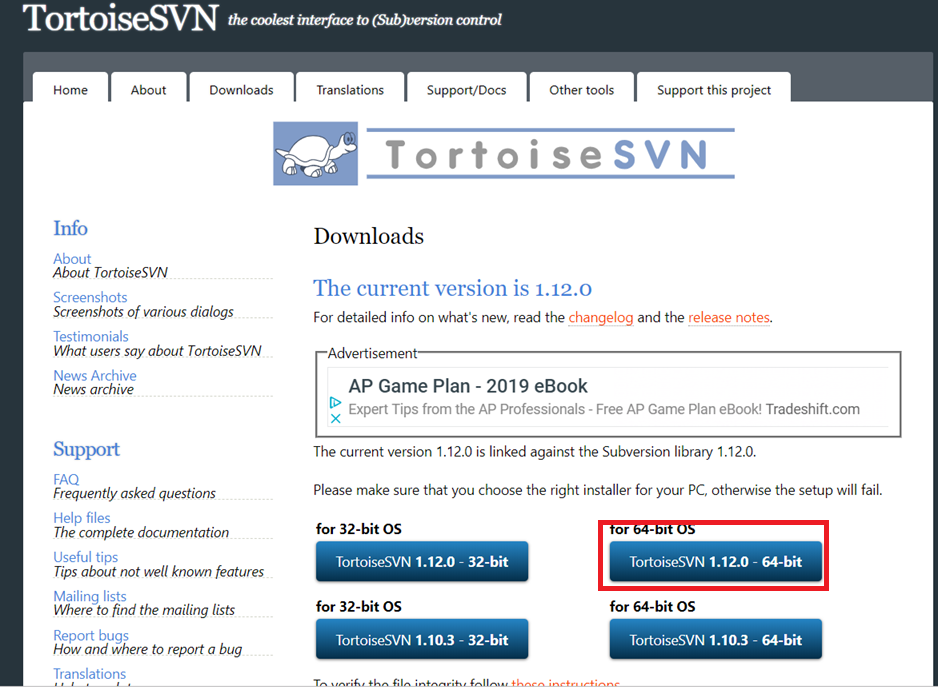
\includegraphics[width=0.9\textwidth]{../images/tortoisesvnDownload.png}
%---------------------------------------------------- fin Imprimer ecran du site de telechargement de svn
\begin{frame}
\frametitle{Installation d'outil complémentaire: TortoiseSVN }
\begin{itemize}
\item Télécharger un installateur en fonction de votre version de Windows( TortoiseSVN 1.12.0 -64-bit) 
\item Aller dans votre dossier de téléchargement Windows 
\item Double cliquer sur l'installateur
\end{itemize}
\end{frame}

\begin{frame}
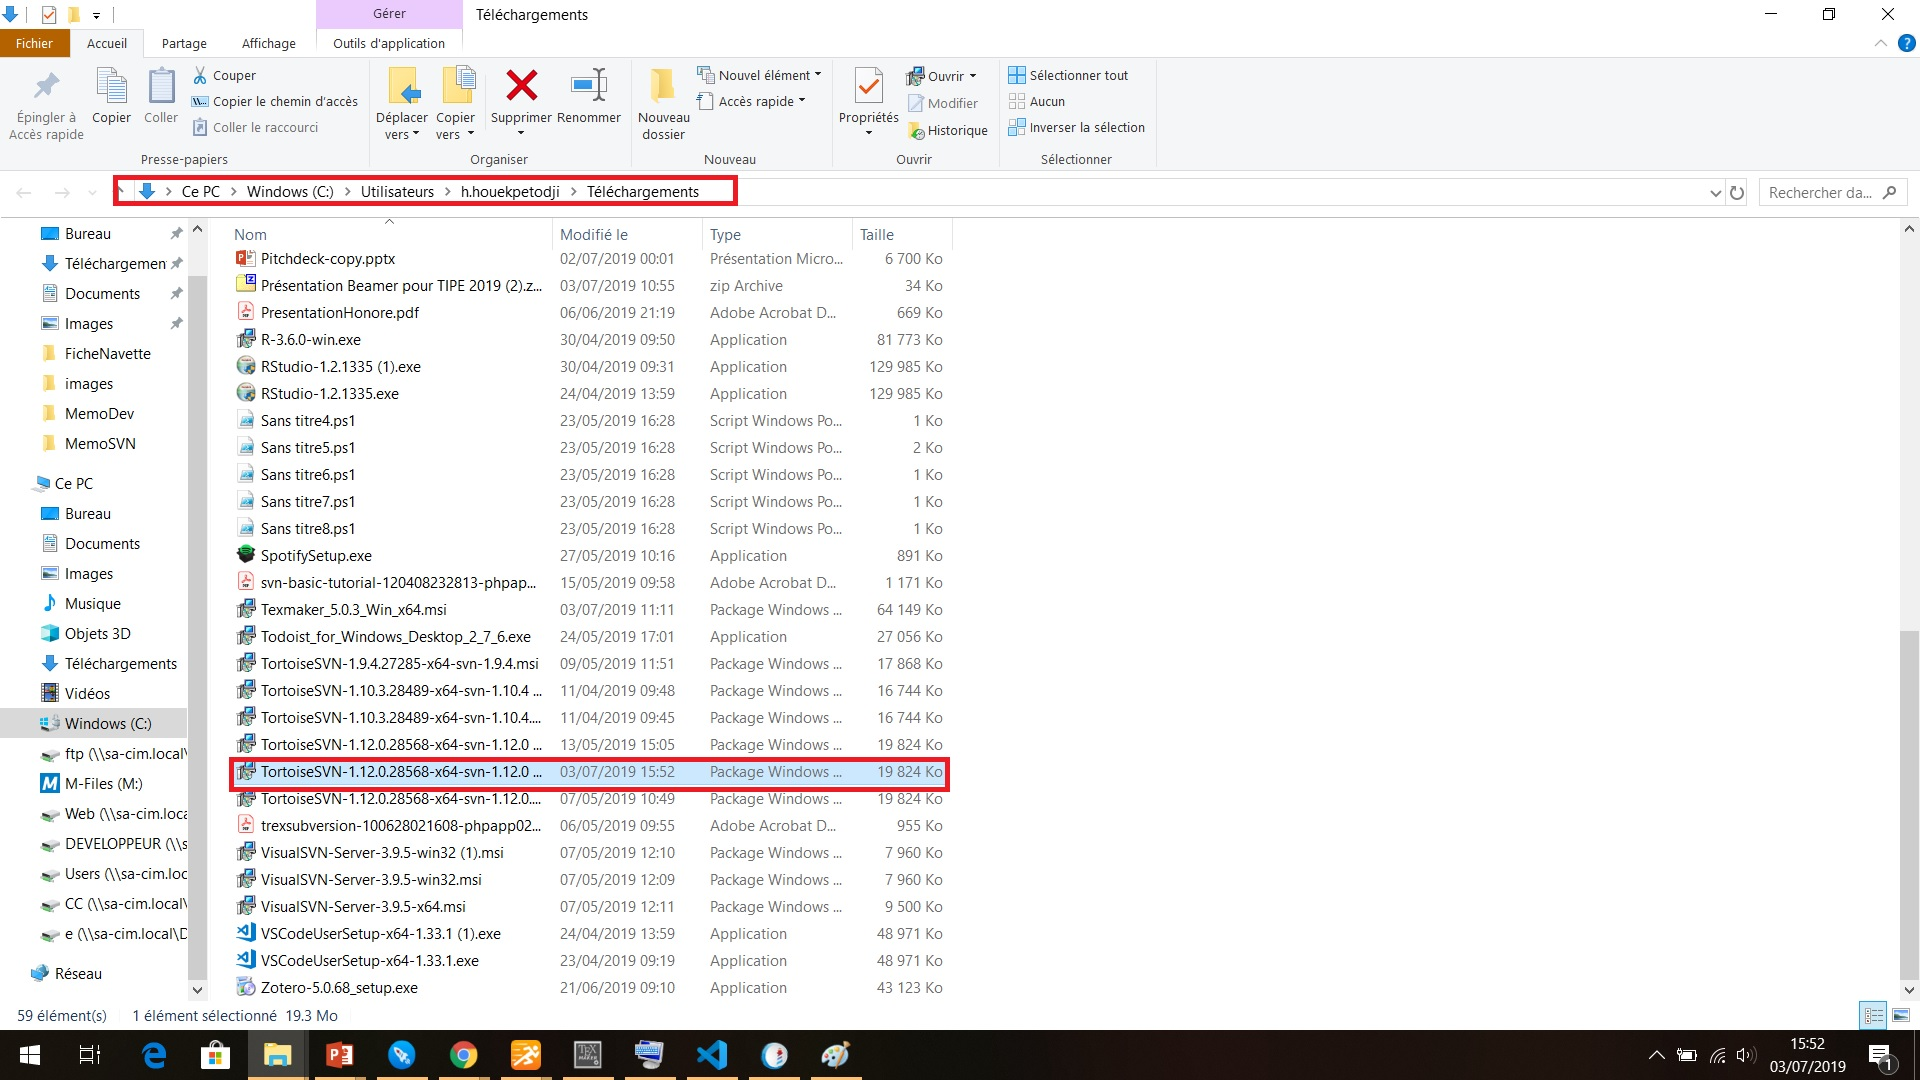
\includegraphics[width=\textwidth]{../images/tortoiseSvnDownloded.jpg}
\end{frame}

\begin{frame}
\frametitle{Installation d'outil complémentaire: TortoiseSVN}
  \begin{columns}[T]
    \begin{column}{.4\textwidth}
     \begin{block}{Étape 1}
Cliquer sur le Bouton \alert{Next}
    \end{block}
     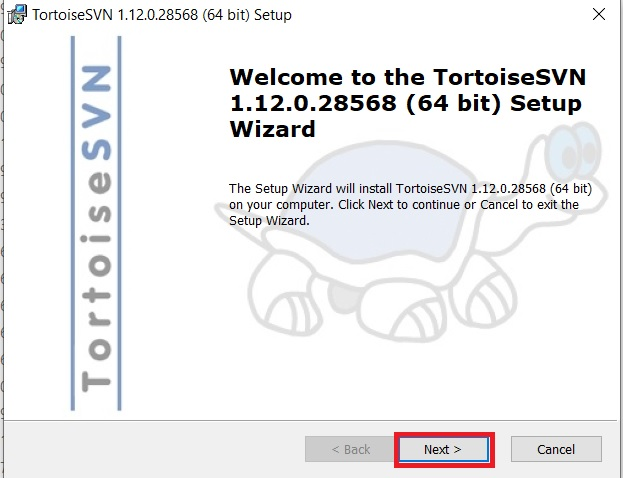
\includegraphics[width=\textwidth]{../images/intalstp1.jpg}
    \end{column}
    \begin{column}{.4\textwidth}
     \begin{block}{Étape 2}
Cliquer sur le Bouton \alert{Next}
    \end{block}
     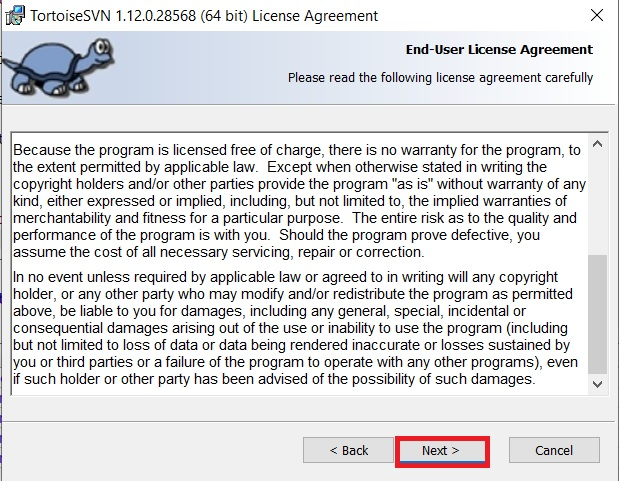
\includegraphics[width=\textwidth]{../images/intalstp2.jpg}
    \end{column}
  \end{columns}
\end{frame}

\begin{frame}
\frametitle{Installation d'outil complémentaire: TortoiseSVN}
  \begin{columns}[T]
    \begin{column}{.4\textwidth}
     \begin{block}{Étape 3}
Cliquer sur le Bouton \alert{Next}
    \end{block}
     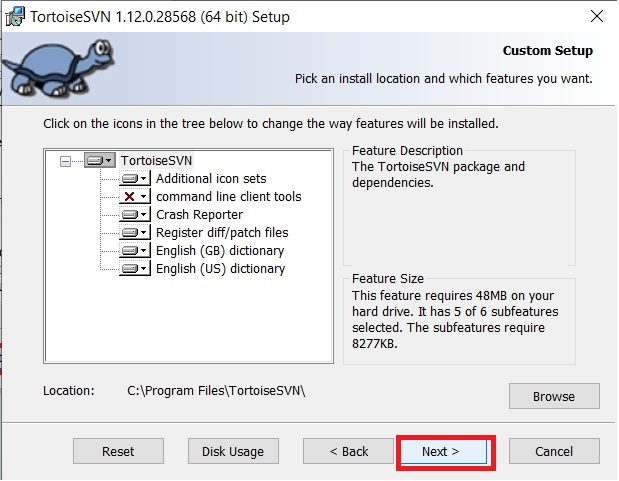
\includegraphics[width=\textwidth]{../images/intalstp3.jpg}
    \end{column}
    \begin{column}{.4\textwidth}
     \begin{block}{Étape 4}
Cliquer sur le Bouton \alert{Next}
    \end{block}
     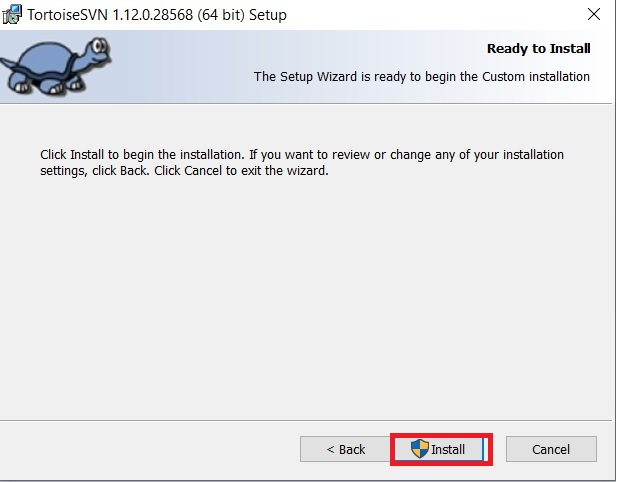
\includegraphics[width=\textwidth]{../images/intalstp4.jpg}
    \end{column}
  \end{columns}
\end{frame}
%---------------------------------------------------------

\section{Introduction au \alert{S}ystème de  \alert{C}ontrôle de \alert{V}ersion \alert{SCV}}

%---------------------------------------------------------
%Highlighting text
\begin{frame}
\frametitle{Utilités d'un SCV}

\begin{columns}[T]
\begin{column}{.7\textwidth}
\begin{block}{Partage de code}
\begin{itemize}
\item Partager votre code avec d’autres personnes
\item Laisser d’autres personnes partager du code avec vous
\end{itemize}
\end{block}
\end{column}
\begin{column}{.4\textwidth}
\begin{center}
  
\includegraphics[width=0.5\textwidth]{../images/travailColaborative.png}
  \end{center}
\end{column}
\end{columns}

\end{frame}

\begin{frame}
\frametitle{Utilitées d'un SCV}

\begin{block}{Voir les changements}
\begin{itemize}
\item Voir les changements effectués dans le code.
\item Savoir qui a fait un changement dans le code.
\item Connaître quand un changement spécifique à été fait
\item Savoir pourquoi un changement a été effectué (commentaires)
\item  Détecter quel changement dans le code a cassé une fonctionnalité
\end{itemize}
\end{block}
\end{frame}
\begin{figure}
 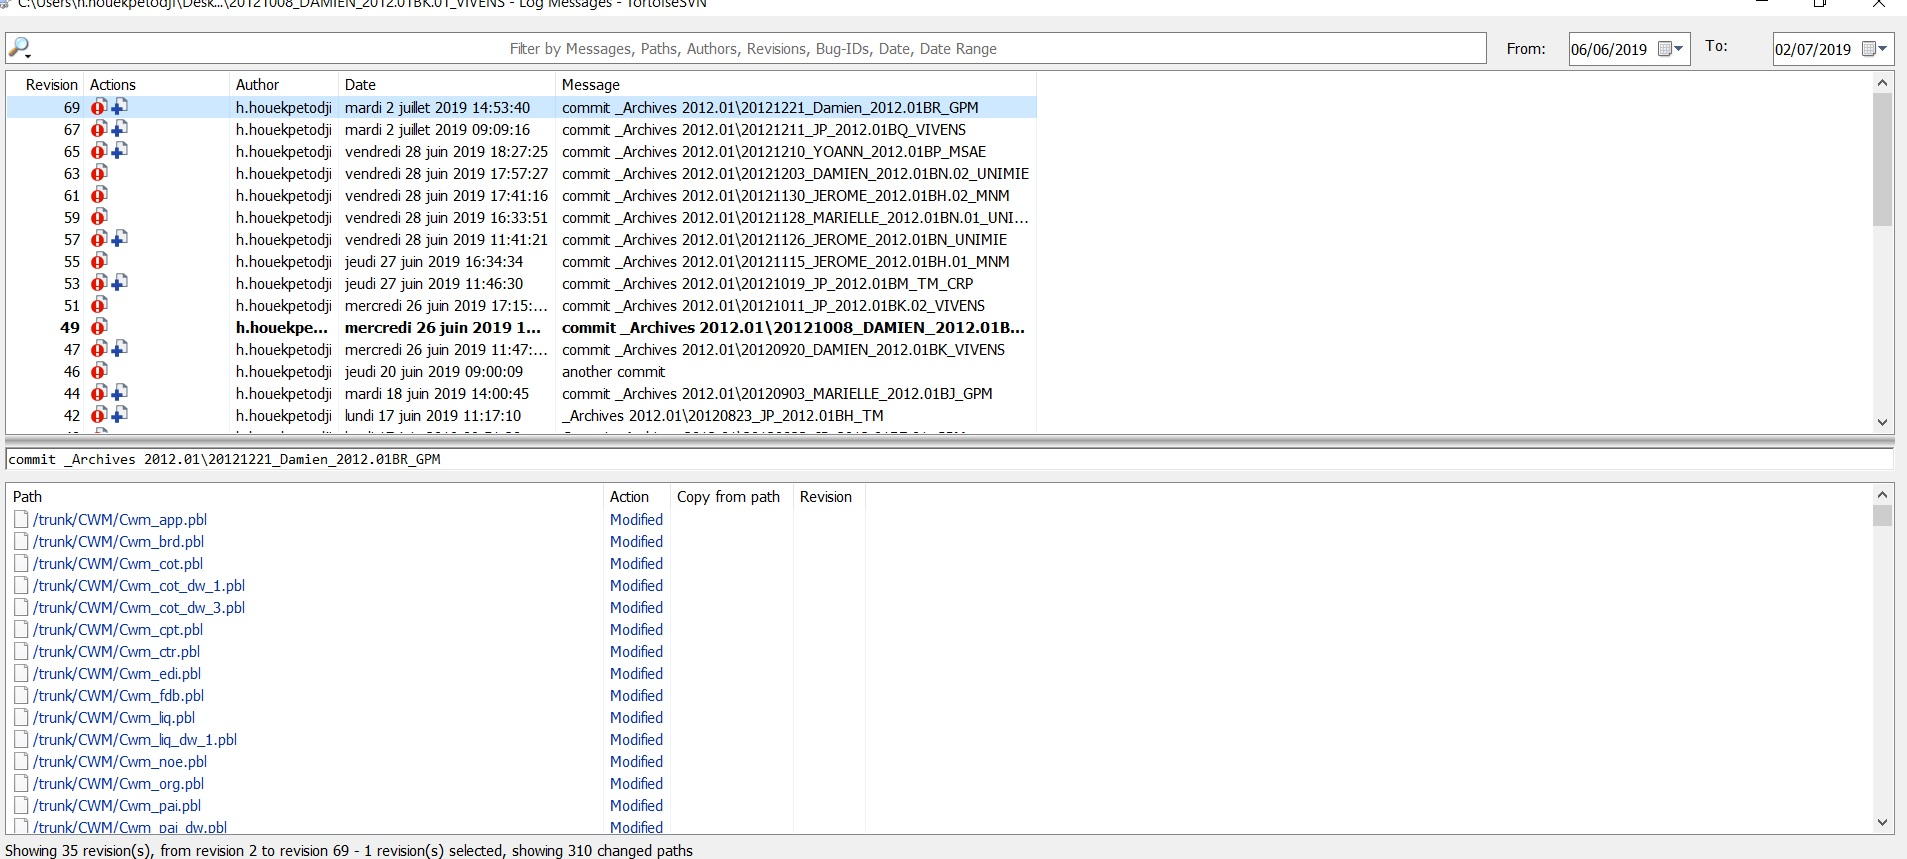
\includegraphics[width=\textwidth]{../images/history.jpg}
 \caption{Historique des changements sur un projet avec subversion}
 \end{figure}

\begin{frame}
\frametitle{Utilitées d'un SCV}
\begin{block}{}
\begin{itemize}
\item Comparer deux versions du code
\end{itemize}
\end{block}
\begin{figure}
 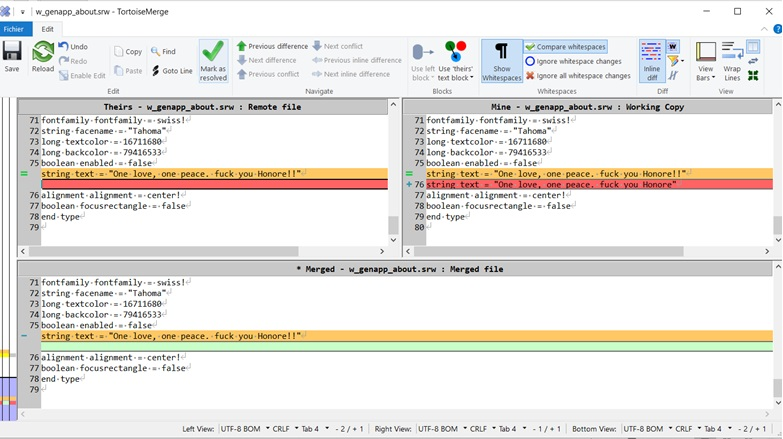
\includegraphics[width=.8\textwidth]{../images/changement.jpg}
 \caption{Comparaison de deux versions d'un projet avec subversion}
 \label{fig:changement}
\end{figure}
\end{frame}
\begin{frame}
\frametitle{Utilitées d'un SCV}
\begin{columns}[T]
\begin{column}{.7\textwidth}
\begin{block}{Maintenance de livrable}
\begin{itemize}
\item Maintenir plusieurs versions d’un produit
\item Fixer un bug sur une version sans livrer de nouvelles fonctionnalités
\end{itemize}
\end{block}
\end{column}

\begin{column}{.3\textwidth}
 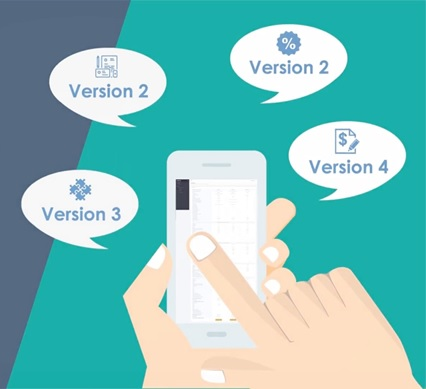
\includegraphics[width=\textwidth]{../images/livrable.jpg}
\end{column}
\end{columns}
\end{frame}
%---------------------------------------------------------


%---------------------------------------------------------
\section{Vocabulaire de base}
\begin{frame}
\frametitle{Vocabulaire}
Pour l'utilisation d'un système de contrôle de version, il y a des termes de base qu'il faut connaitre. Ces termes sont: version, révision, patch, diff, dépôt, copie locale, branche, fusion de branche, conflit, étiquetage ou marquage, mise à jour. Dans la suite nous allons définir ces termes.
\end{frame}
\begin{frame}
\frametitle{Vocabulaire}
\begin{block}{Version}
Pour un logiciel qui évolue, chaque étape de son évolution est appelée \alert{version} ou \alert{révision}. Toutes les \alert{versions} sont liées à travers des modifications appelées \alert{patch} ou \alert{diff}. Le numéro de version est incrémenté automatiquement après modification. On a:
$ version_{N+1}=  modification(version_N) $
\end{block}

\end{frame}
\begin{frame}
\frametitle{Vocabulaire}
\begin{block}{Depôt et copie locale}
Les fichiers versionnés sont mis à disposition dans un espace de stockage public géré par un logiciel de contrôle de version(\alert{dépôt}). Pour pouvoir effectuer des modifications, le développeur doit d'abord faire une \alert{copie locale} des fichiers qu'il souhaite modifier, ou de tout le dépôt. 
\end{block}

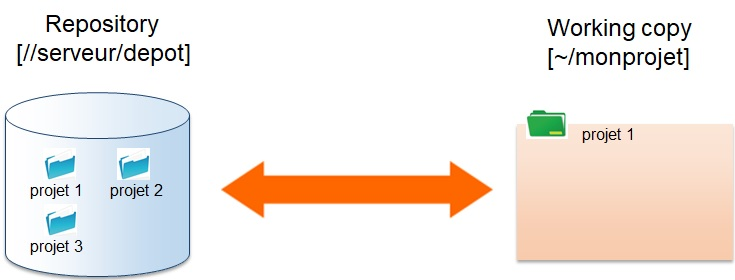
\includegraphics[width=.7\textwidth]{../images/depot.jpg}
\end{frame}
\begin{frame}
\frametitle{Vocabulaire}
\begin{block}{Branche}
Une branche est crée lorsqu'on veux diverger de la ligne principale de développement et continuer à travailler sans se préoccuper de cette ligne principale. Le fait de vouloir rassembler deux branches est \alert{une fusion de branches}. Les branches sont utilisées pour permettre :
\begin{itemize}
\item la maintenance d'anciennes versions du logiciel (sur les branches) tout en continuant le développement des futures versions (la ligne principale) ;
\item le développement parallèle de plusieurs fonctionnalités volumineuses sans bloquer le travail quotidien sur les autres fonctionnalités.
\end{itemize}

\end{block}

\end{frame}
\begin{frame}
\frametitle{Vocabulaire}
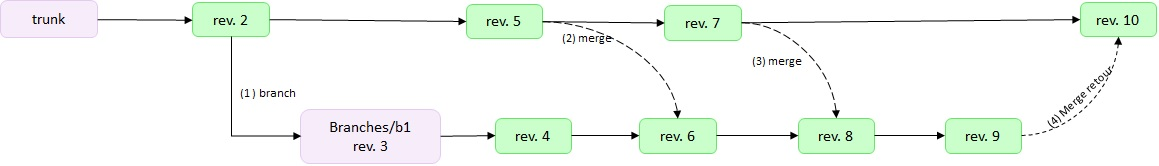
\includegraphics[width=\textwidth]{../images/branche.jpg}\\
\end{frame}

\begin{frame}
\frametitle{Vocabulaire}
Dans le cas d'un développement en équipe, les tâches sont reparties entre développeurs. Il est nécessaire de partager une base commune de travail. C'est tout l'intérêt des systèmes de gestion de version.
\begin{block}{Conflit de modifications}
 Quand deux ou plusieurs développeurs modifient en même temps la  même partie d'un fichier. Dans ce cas on parle alors de \alert{conflit de modifications}. Le système de contrôle de version ne sait pas quelle modification il faut appliquer
\end{block}
\end{frame}

\begin{frame}
\frametitle{Vocabulaire}
\begin{block}{Conflit de modifications}
Les SCVs  intègrent les outils de \alert{diff/merge}. Le développeur peut voir et comparer les versions en conflit. Ces outils lui permettent de choisir la version qu'il souhaite garder.
\end{block}
 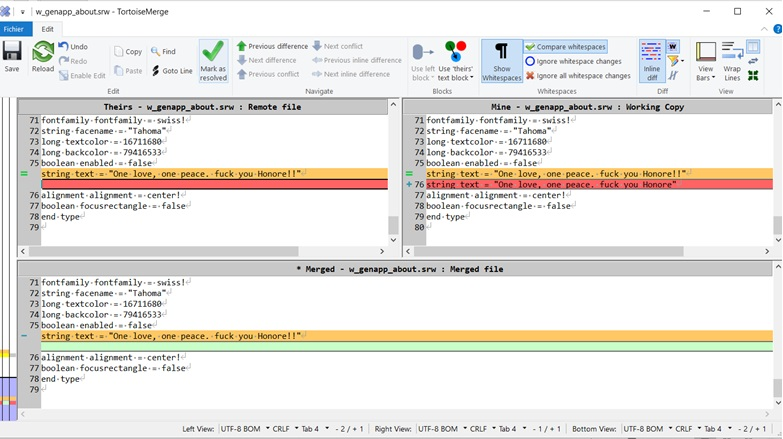
\includegraphics[scale=.5]{../images/changement.jpg}

\end{frame}
\begin{frame}
\frametitle{Vocabulaire}
\begin{block}{Étiquetage ou marquage}
L'étiquetage consiste à associer un nom à une version donnée. C'est un moyen de retrouver facilement une version significative. Elle est appelée \alert{tag}
\end{block}
 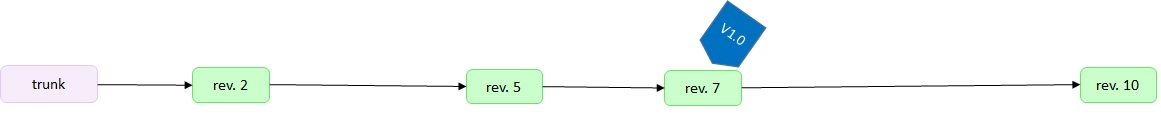
\includegraphics[scale=0.5]{../images/etiquetage.jpg}
\end{frame}

\begin{frame}
\frametitle{Vocabulaire}
\begin{block}{Mise à jour}
On distingue deux types de mise à jour.
\begin{enumerate}
\item La mise à jour de la copie locale depuis le dépôt :  \alert{update}. Cette opération consiste à récupérer les dernières modifications subvenues sur le projet depuis le dépôt. 
 \item La mise à jour de la version du dépôt depuis sa copie locale :  \alert{commit}. Cette opération consiste à mettre ces modifications dans le dépôt du système de contrôle de version.
\end{enumerate}
\end{block}
\end{frame}
%---------------------------------------------------------
\begin{frame}
Il existe plusieurs système de contrôle de version. On peut citer entre autres: \alert{Subversion SVN}, CVS, Git, GNU Arch,etc. \alert{SVN} est simple d'utilisation. 
\end{frame}

\section{Présentation de SVN}
\begin{frame}
\frametitle{Presentation de SVN}
\begin{block}{Bonne pratiques avec SVN}
\begin{itemize}
\item Pour faciliter la gestion d'un projet avec SVN, il faut définir trois répertoire de base à savoir:
\begin{enumerate}
\item \alert{Trunk : } il contient la ligne principale du projet. La dernière version du projet doit toujours être dans ce répertoire. Il peut contenir par exemple la version évolutive d'IzyProtect.
\item \alert{Tags : } ce répertoire est dédié pour les livrables. Il est fortement déconseillé d'ajouter les modifications directement à cet répertoire. En résumer il contient que \alert{les versions étiquetées}. Dans le cadre de CIM c'est les versions arrêtées nommées et datée. Exemple: \alert{\textit{20190628\_MANU\_2017.01AO.01QUATER}} 
\item \alert{Branches : } Ce répertoire contient la version de développement du projet. Il permet de développer de nouvelle fonctionnalités. Les bugs fix  ont aussi lieu dans ce répertoire. 
\end{enumerate}
\end{itemize}

\end{block}
\end{frame}

\begin{frame}
\frametitle{Presentation de SVN}
\begin{block}{Bonne pratiques avec SVN}
\begin{itemize}
\item  Il est fortement déconseillé de faire un \alert{SVN commit  d’une fonctionnalité cassée}.
\item \alert{Tester obligatoirement le projet} avant de faire l’opération SVN commit
\item Toujours faire une opération de  \alert{SVN update} avant de commencer à travailler. 
 
\end{itemize}
\end{block}
\end{frame}

\begin{frame}
\frametitle{Presentation de SVN}
\begin{block}{Bonne pratiques avec SVN}
\begin{itemize}
\item Enregistrer  les modifications locales et faire un \alert{SVN update} fréquemment. Ceci permet d'être à jour par rapport aux modifications des autres. Ceci réduit les conflits .
\item Toujours faire  un \alert{SVN commit} régulièrement( par petit grain de modifications). L'avantage est que la résolutions des conflits est moins complexe. 
\end{itemize}
\end{block}
\end{frame}


\section{Utilisation de SVN avec PowerBuilder}

\begin{frame}
\frametitle{Pré-requis}
\begin{block}{Pré-requis}
Pour commencer à travailler avec SVN. Il faut préparer l'environnement de travail (voir slide ~\ref{preparation}). Il faut aussi un \alert{URL} vers le projet qui sera fourni par l'administrateur du SVN.
\end{block}
\end{frame}

%\begin{frame}
%\frametitle{Icônes sur les objets et leurs significations}
%\begin{table}
%\begin{tabular}{ | l | c | }
%\hline
%Icones & Signification sur l'objet qui le porte  \\
%\hline 
%
\includegraphics[scale=0.2]{../images/sccicon1.png}\\
% & 13:04 \\ 
%\hline 
%Norman P & 8:00\\
%\hline 
%Alex K & 14:00 \\
%\hline 
%Sarah H & 9:22 \\
%\hline 
%\end{tabular}
%\caption{Triathlon results}
%\end{table}
%\end{frame}
%
%\begin{frame}
%\begin{center}
%\huge{Récupération d'un projet}
%\end{center}
%\end{frame}


\begin{frame}
\frametitle{PowerBuilder}
\begin{block}{Récupération d'un projet}
\begin{itemize}
\item copier et coller l'URL du projet dans le champ \alert{\textit{Repository URL}}
\item saisir son identifiant et son mot de passe respectivement dans les champs \alert{\textit{User ID , Password}}
\item choisir un dossier vide où PowerBuilder va mettre le projet dans le champ \alert{\textit{Checkout Directory}}
\item cliquer sur le boutton \alert{\textit{ok}}. 
\end{itemize}
\end{block}
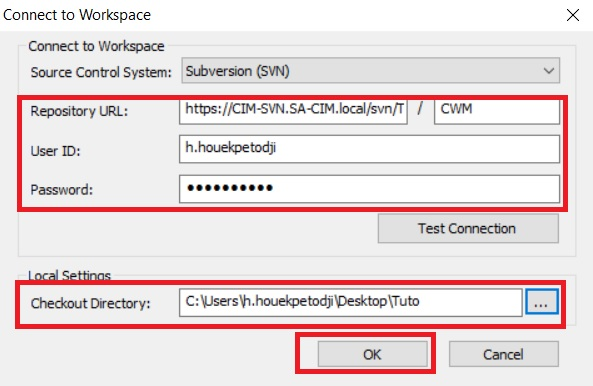
\includegraphics[scale=0.4]{../images/connect2.jpg}
\end{frame}
\begin{frame} 
\frametitle{PowerBuilder}
\begin{block}{Récupération d'un projet}
Une fois la récupération du projet terminée. Le projet est ouvert dans votre espace de travail PowerBuilder. Vous êtes prêt pour ajouter vos modifications. Votre écran ressemblera à ça:

\end{block}
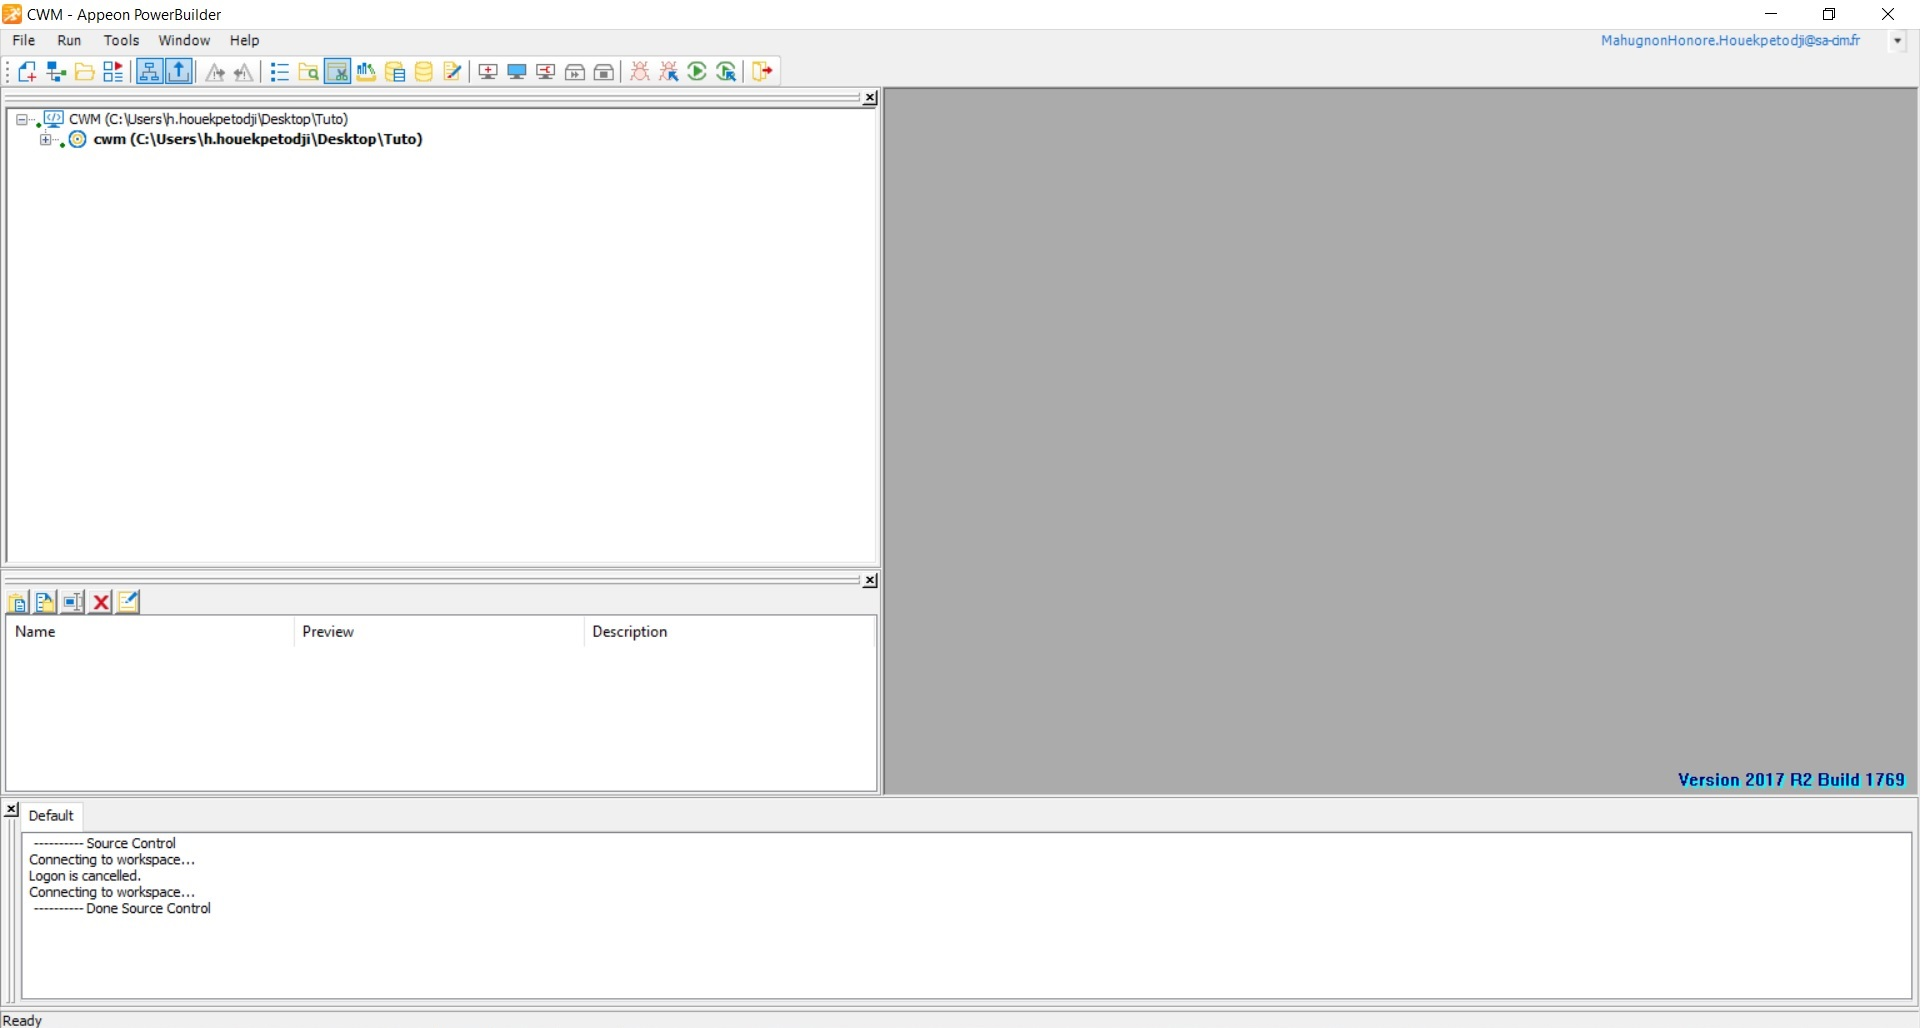
\includegraphics[scale=0.25]{../images/connect3.jpg}
\end{frame}


\begin{frame}
\begin{center}
\huge{Ajout modification}
\end{center}
\end{frame}

\begin{frame}
\frametitle{PowerBuilder}
\begin{block}{Ajout modification}
Nous allons apporter des modifications à notre projet qu'on a récupéré. Dans cet exemple, nous allons modifier un commentaire de la PB function \alert{\textit{cwm\_abc.pbl $\rightarrow$ uf.bitshr}}
\end{block}
 
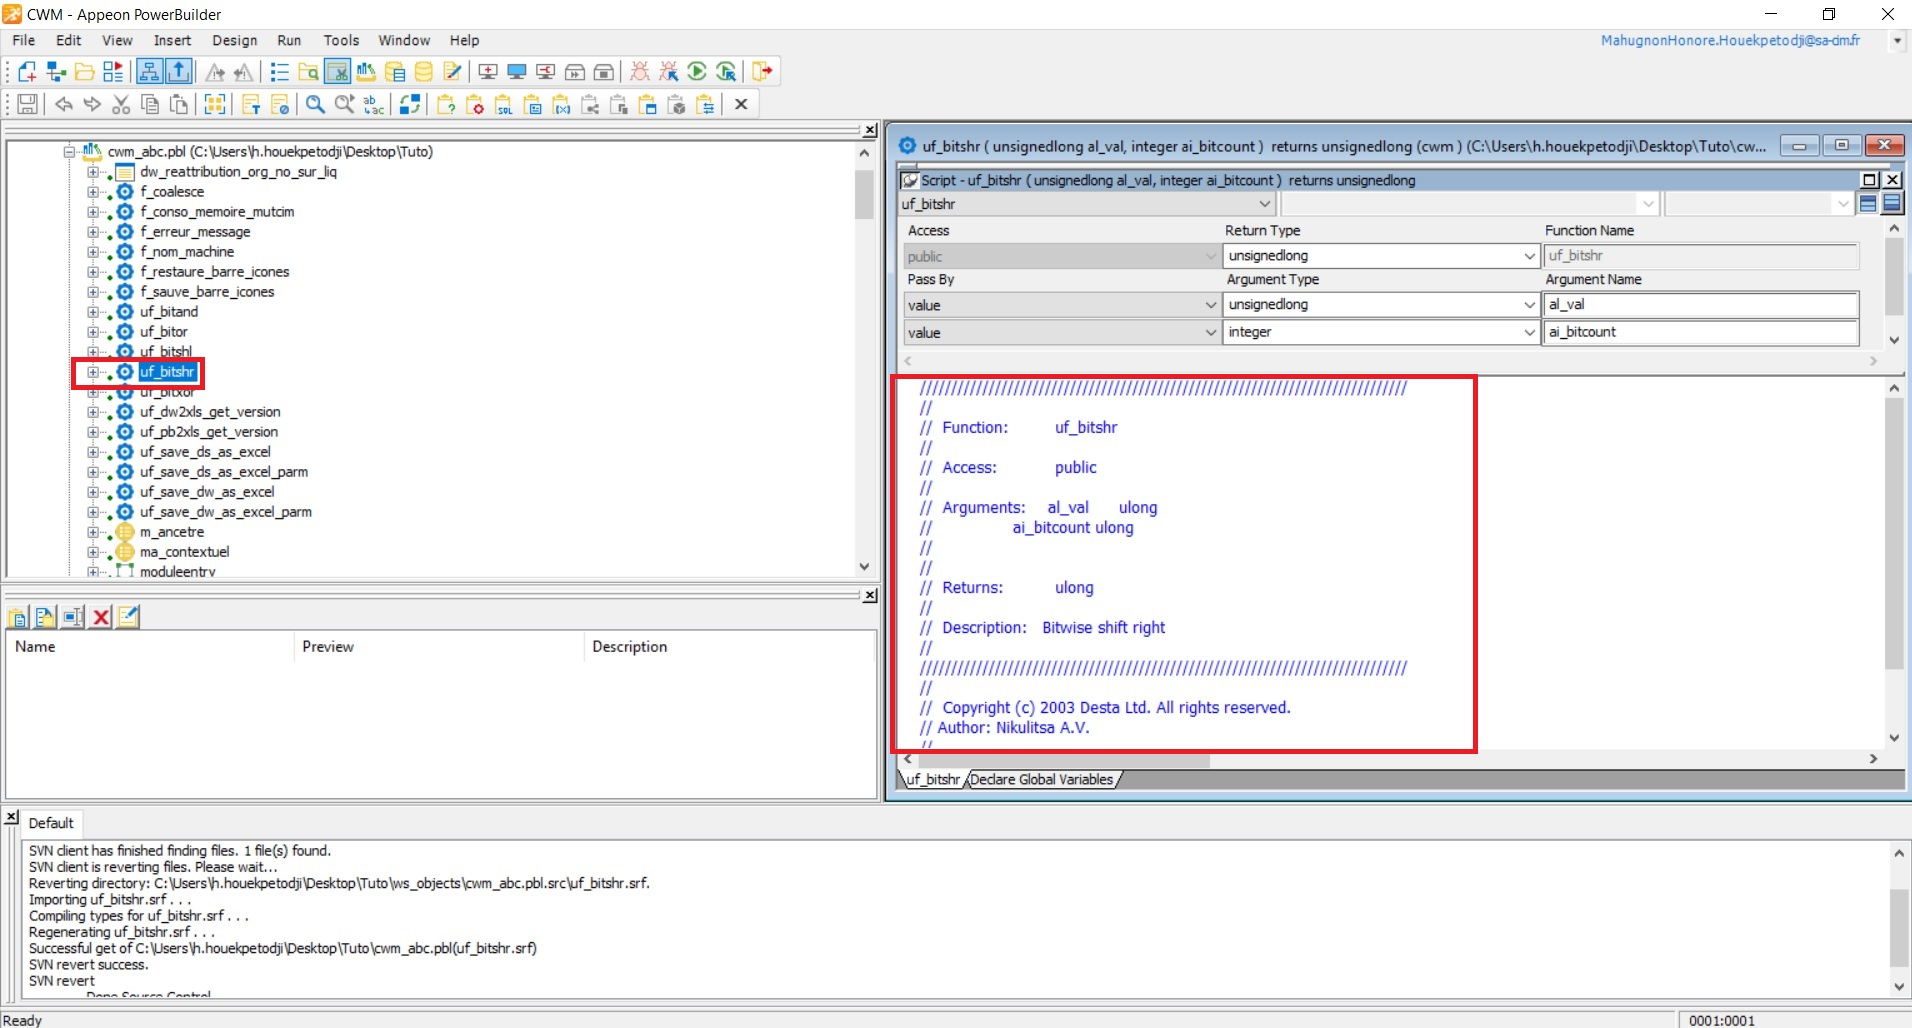
\includegraphics[scale=.2]{../images/modif1.jpg}
\end{frame}

\begin{frame}
\frametitle{PowerBuilder}
\begin{block}{Ajout de modifications}
Après avoir enregistrer nos modifications, on a:
\begin{itemize}
\item Remarquer une pastille verte \scalerel*{
\includegraphics{../images/check.jpg}}{B} à gauche sur l'écran  sur les modifications enregistrées.
\end{itemize}
\end{block}
 
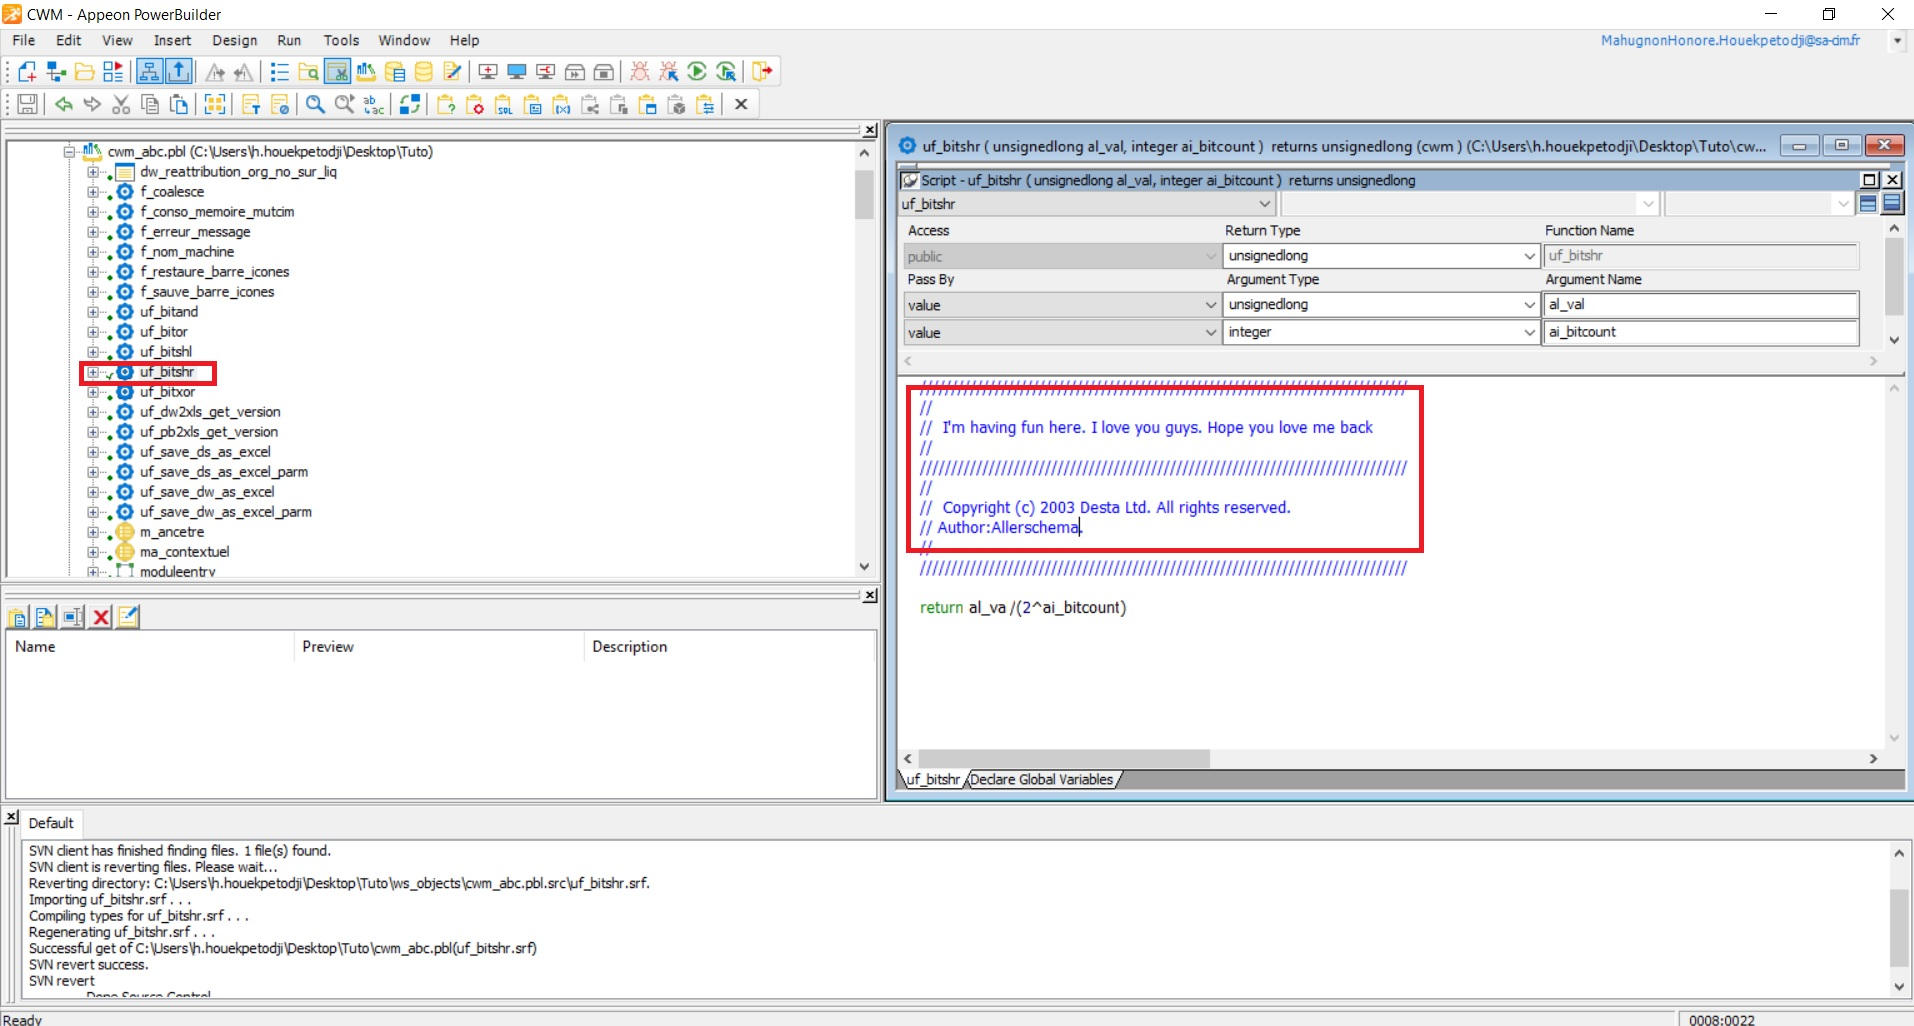
\includegraphics[scale=.2]{../images/modif2.jpg}
\end{frame}

\begin{frame}
\frametitle{PowerBuilder}
\begin{block}{Ajout de modifications}
Une fois les modifications terminées, commiter les modifications dans le dépôt de SVN.  Pour cela :
\begin{itemize}
\item Récupérer les modifications des développeurs via \alert{SVN update}. Cette opération permet d'être à jour. 
\item Tester la mise à jour.
\item commiter effectuées dans le depôt SVN.
\end{itemize} 
\end{block}
\end{frame}

\begin{frame}
\begin{center}
\huge{Mise à jour de la copie locale}
\end{center}
\end{frame}

\begin{frame}
\frametitle{PowerBuilder}
\begin{block}{Mise à jour de la copie locale}
\begin{itemize}
\item Cliquer droit sur le workspace du projet
\item choisir l'option \alert{\textit{SVN update}}
\end{itemize}
\end{block}
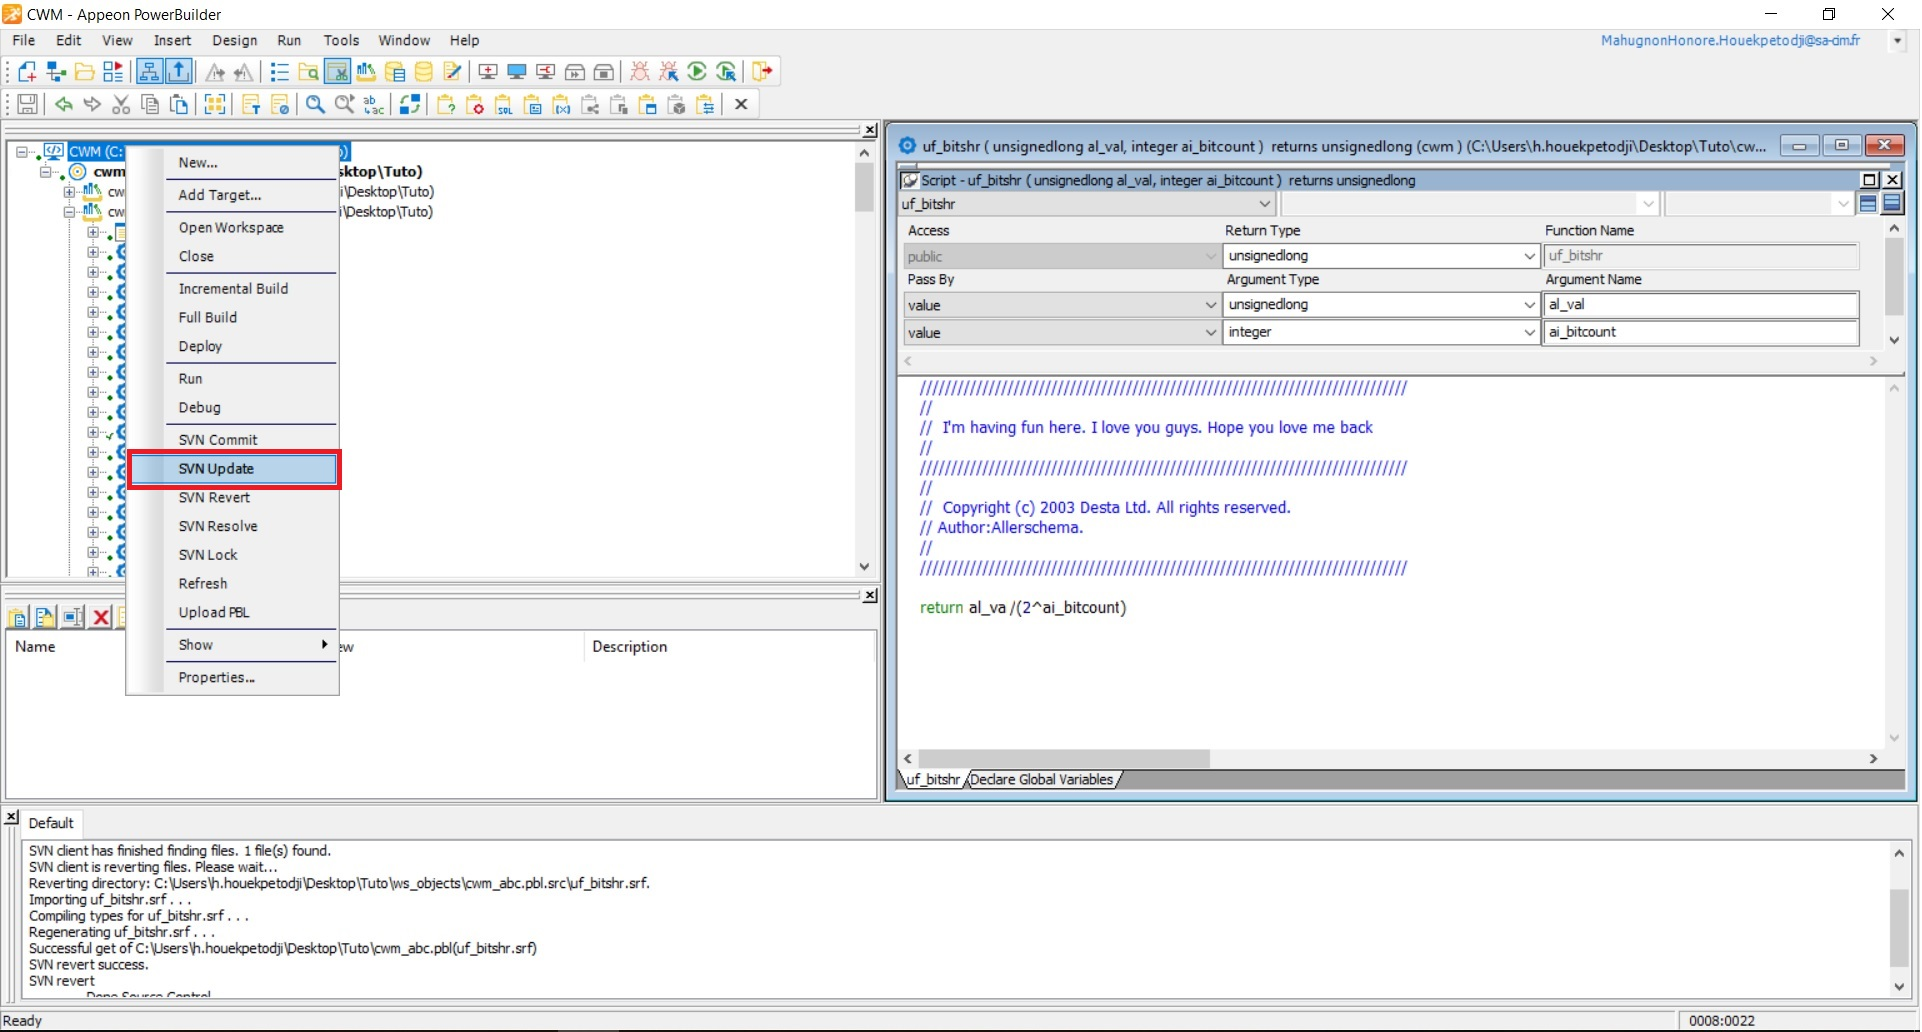
\includegraphics[scale=0.25]{../images/svnupdate.jpg}
\end{frame}

\begin{frame}
\begin{center}
\huge{Commiter les modifications}
\end{center}
\end{frame}

\begin{frame}
\frametitle{PowerBuilder}
\begin{block}{ Commiter les modifications}
\begin{itemize}
\item Cliquer droit sur le workspace du projet
\item choisir l'option \alert{\textit{SVN commit}}
\item Écrire un commentaire qui résume les modifications
\end{itemize} 
\end{block}
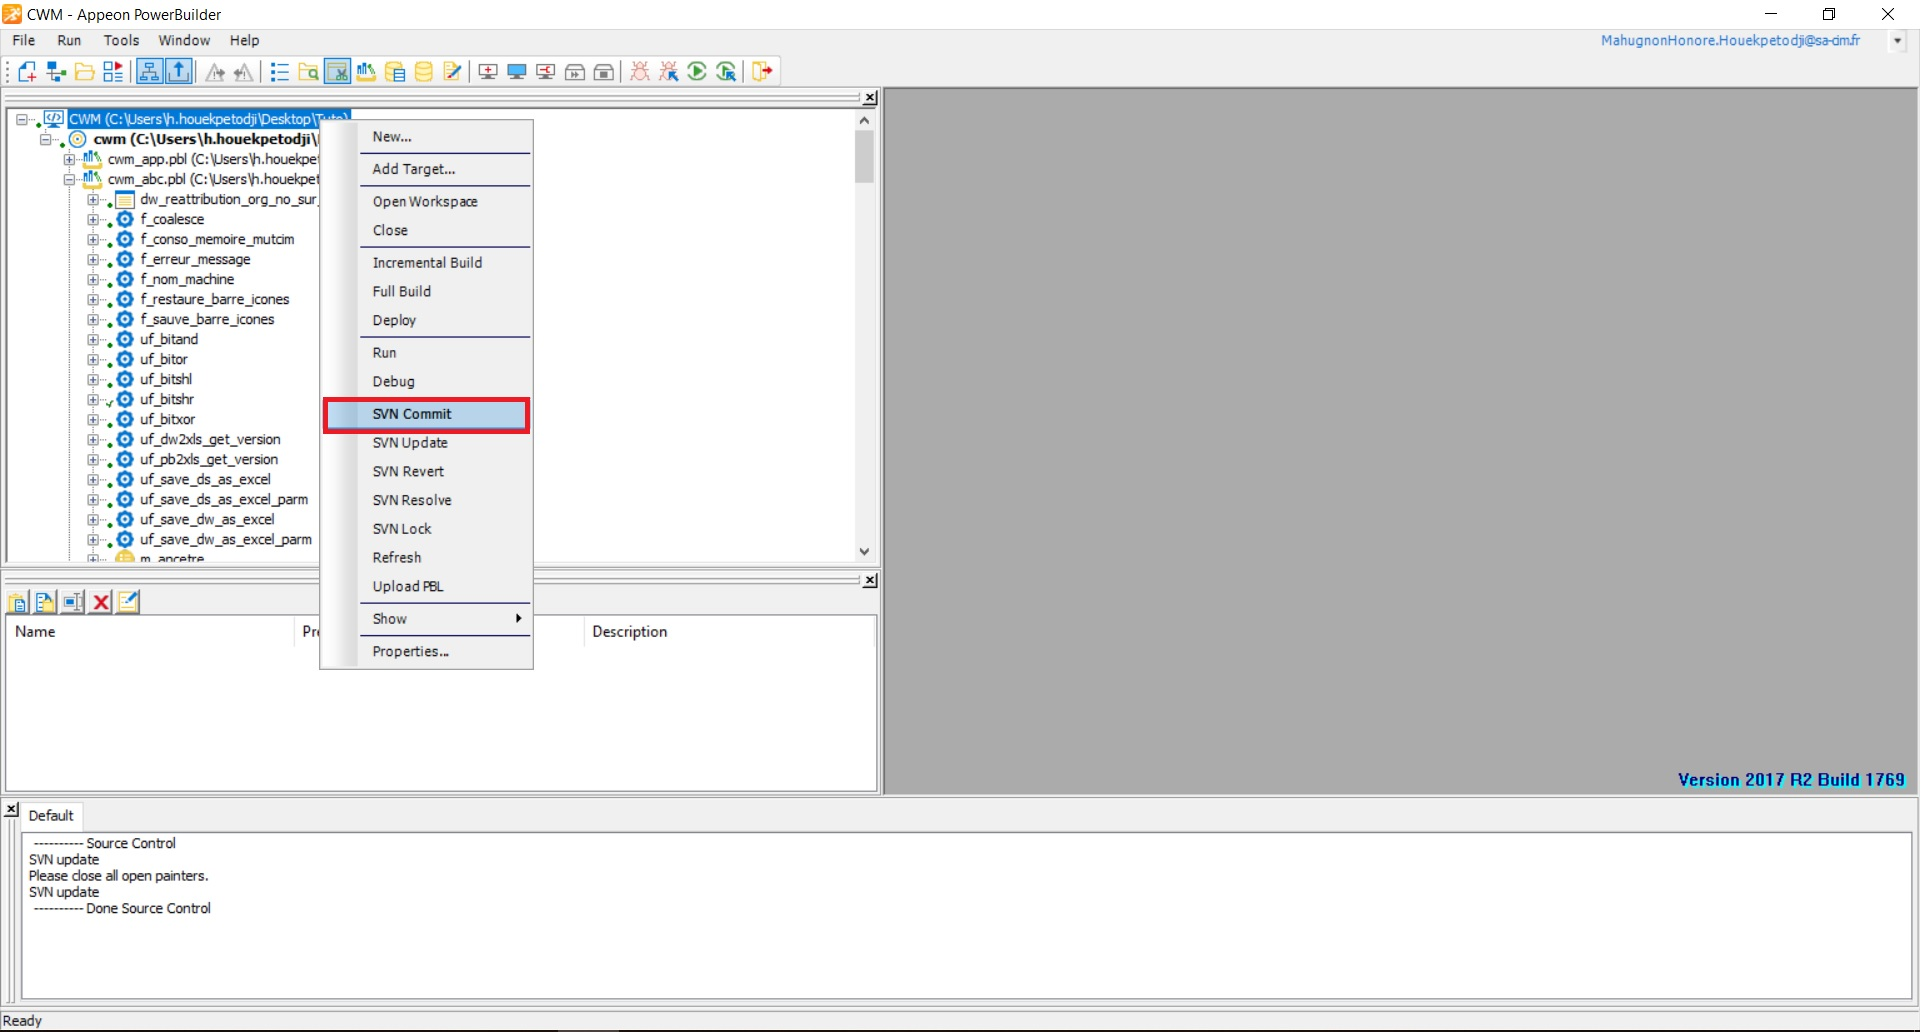
\includegraphics[scale=0.25]{../images/commit1.jpg}
\end{frame}

\begin{frame}
\frametitle{PowerBuilder}
\begin{block}{ Commiter les modifications}
\begin{itemize}
\item Écrire un commentaire qui résume vos modifications
\item Appuyer sur le bouton ok
\end{itemize}

\end{block}
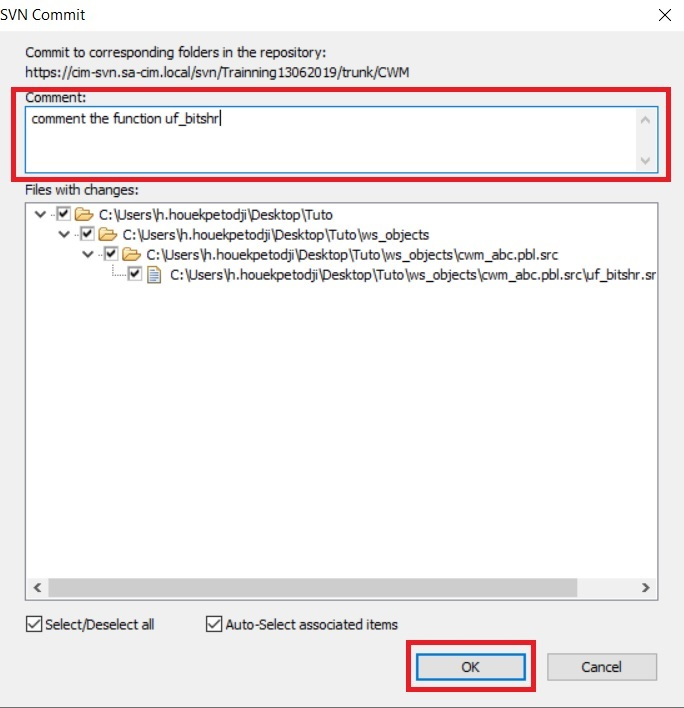
\includegraphics[scale=0.4]{../images/commit4.jpg}
\end{frame}

\begin{frame}
\frametitle{PowerBuilder}
Si l'opération \alert{\textit{SVN commit}} échoue, il faut faire \alert{\textit{SVN update}} et réessayer. Si elle échoue une autre fois, envisager un cas de conflit. La résolution de conflit est supportée par TortoiseSVN. 
\end{frame}

\begin{frame}
\begin{center}
\huge{Annuler modifications}
\end{center}
\end{frame}

\begin{frame}
\frametitle{PowerBuilder}
\begin{block}{ Annuler modifications}
Il arrive des moments où on veut annuler  certains changements. SVN permet d'annuler les changements en local via l'opération \alert{\textit{Revert}}. Dans l'IDE PowerBuilder il faut procéder comme suit:
\begin{itemize}
\item Cliquer  droit sur le changement spécifique à annuler
\item Sélectionner l'option \alert{\textit{SVN Revert}}
\end{itemize}
\end{block}
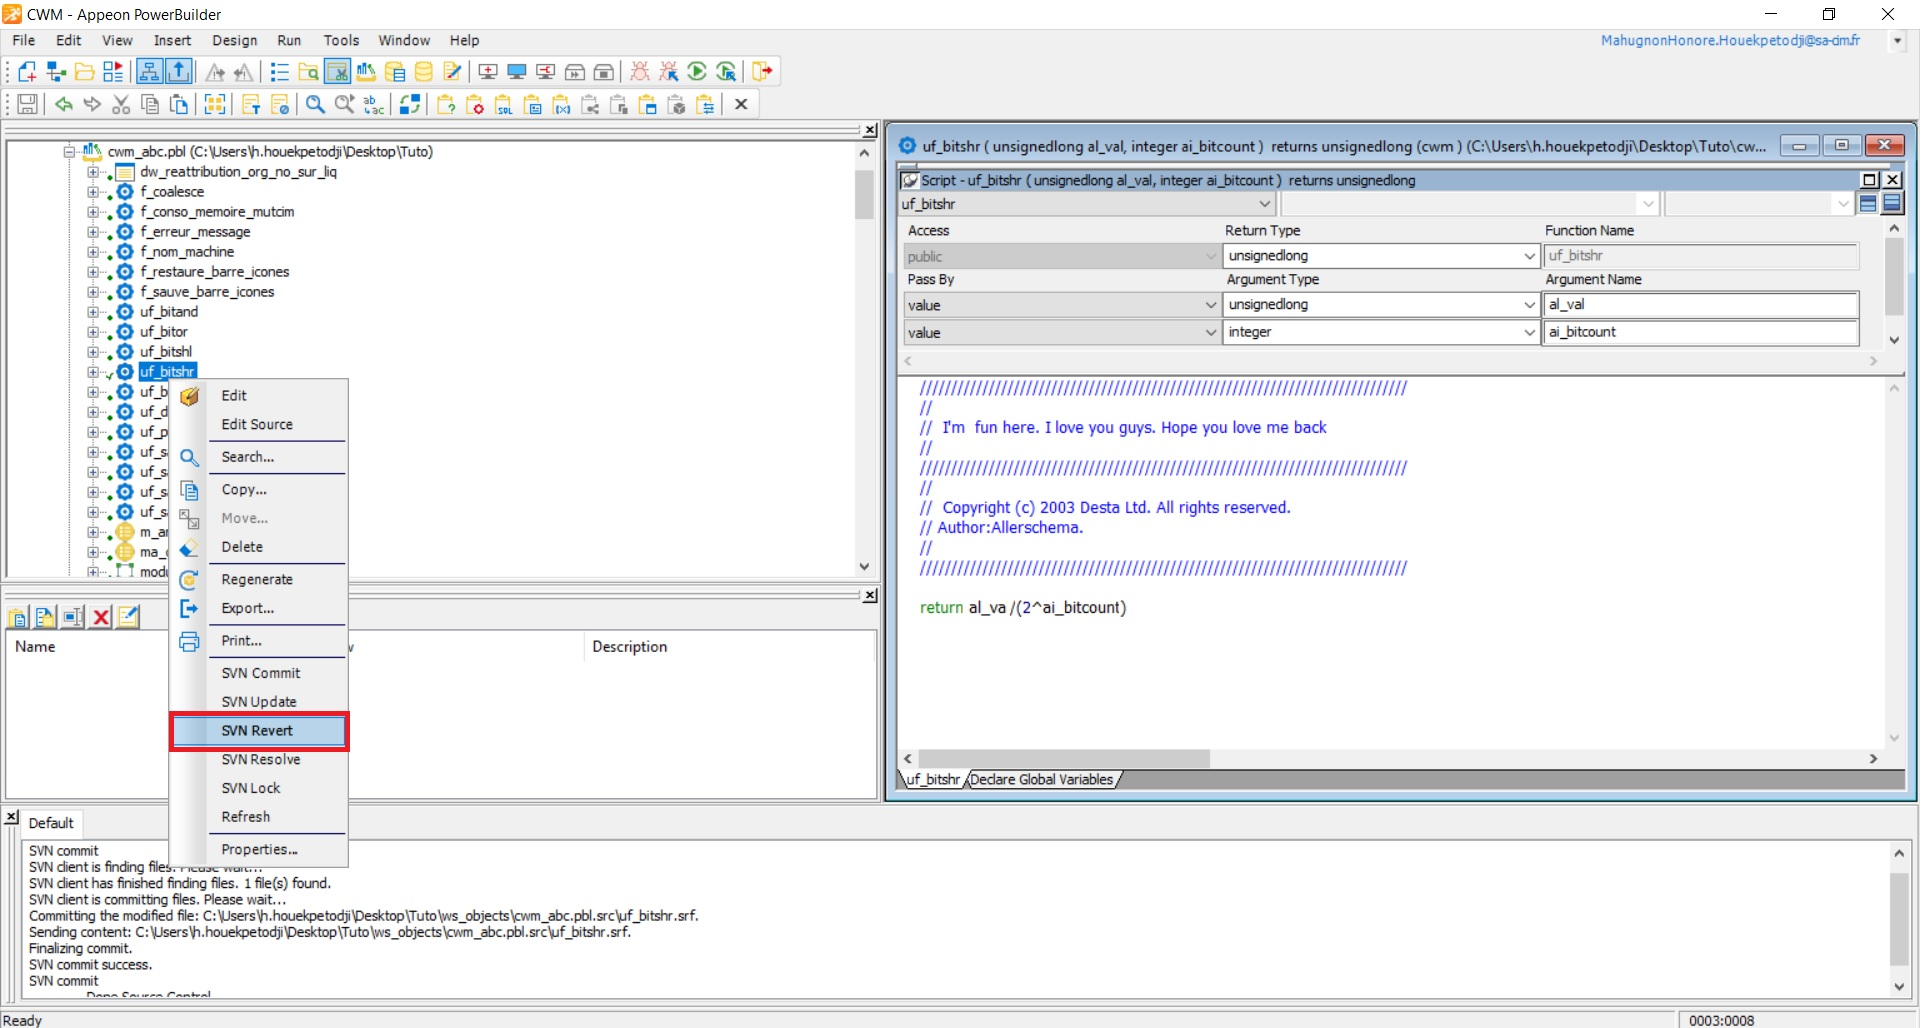
\includegraphics[scale=0.2]{../images/annulerM.jpg}
\end{frame}

\begin{frame}{PowerBuilder }
L'IDE PowerBuilder  propose une intégration avec SVN. Mais PowerBuilder fournit des commandes très limitées. Dans ce sens, il faut utiliser en complément l'outil \alert{TortoiseSVN}. 
\end{frame}

\section{Utilisation de SVN avec TortoiseSVN}

\begin{frame}
\frametitle{Utilisation de TortoiseSVN}
Dans cette partie, nous supposons que TortoiseSVN a été  installé sur votre machine. Si ce n'est pas le cas, veuillez suivre le slide ~\ref{preparation}.
 Voici les icônes de TortoiseSVN et leurs significations.
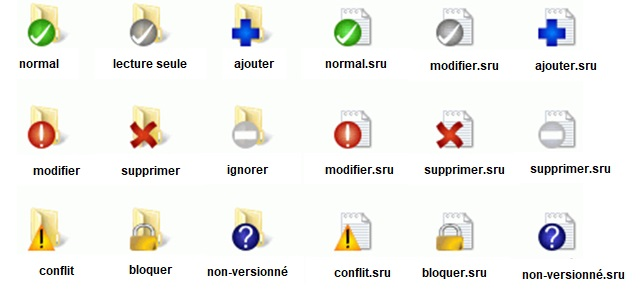
\includegraphics[scale=.7]{../images/icon.jpg} 
\end{frame}

\begin{frame}
\begin{center}
\huge{Récupérer un projet depuis le dépôt SVN}
\end{center}
\end{frame}

\begin{frame}
\frametitle[\label{chekout}]{Utilisation de TortoiseSVN}
\begin{block}{Récupérer un projet depuis le dépôt SVN }
L'action de récupération de projet depuis le dépôt SVN est appelé :  \alert{\textit{Checkout}}. Avec TortoiseSVN, il faut disposer de l'URL vers le projet dans le dépôt SVN. L'URL est fournit par le manager du projet. De plus il faut un dossier vide dans lequel TortoiseSVN va mettre le projet.  Ensuite, il faut
\begin{itemize}
\item Cliquer droit n'importe où dans Windows et choisir l'option \alert{\textit{SVN Checkout}}.
\end{itemize}
\end{block}
\end{frame}
\begin{frame}
\frametitle{Utilisation de TortoiseSVN}
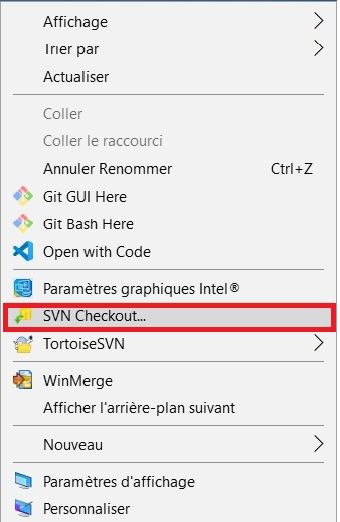
\includegraphics[scale=0.25]{../images/checkout1.jpg}
\begin{block}{Récupérer un projet }

\begin{itemize}
\item Spécifier respectivement, l'URL du projet et le dossier destination
\end{itemize}
\end{block}
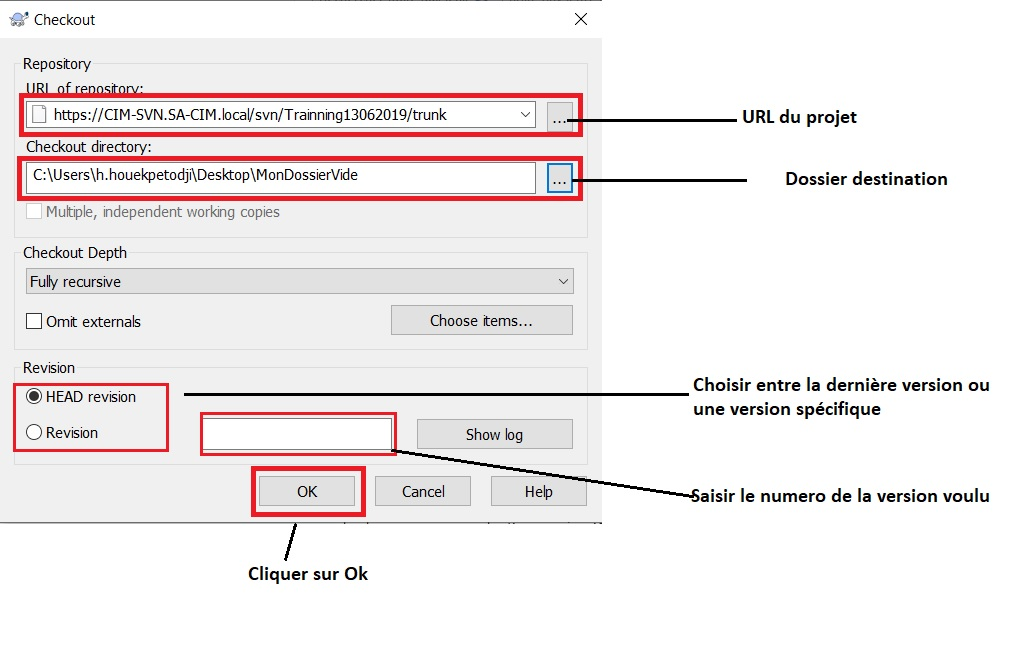
\includegraphics[scale=0.25]{../images/checkout2.jpg}
\end{frame}
\begin{frame}
\frametitle{Utilisation de TortoiseSVN}
\begin{block}{Récupérer un projet depuis le dépôt SVN }
\begin{itemize}
\item Patienter un peu
\item Cliquer sur ok
\end{itemize}
\end{block}
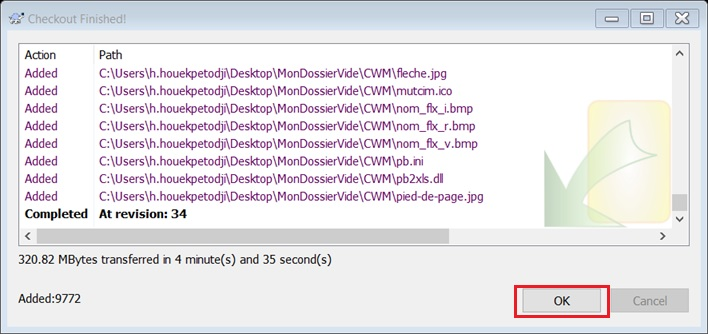
\includegraphics[scale=0.3]{../images/checkout3.jpg}
\newline
\newline
\newline
Finalement le dossier initialement vide contient le projet.
\end{frame}

\begin{frame}
\begin{center}
\huge{Commiter les modifications}
\end{center}
\end{frame}

\begin{frame}
\frametitle{Utilisation de TortoiseSVN}
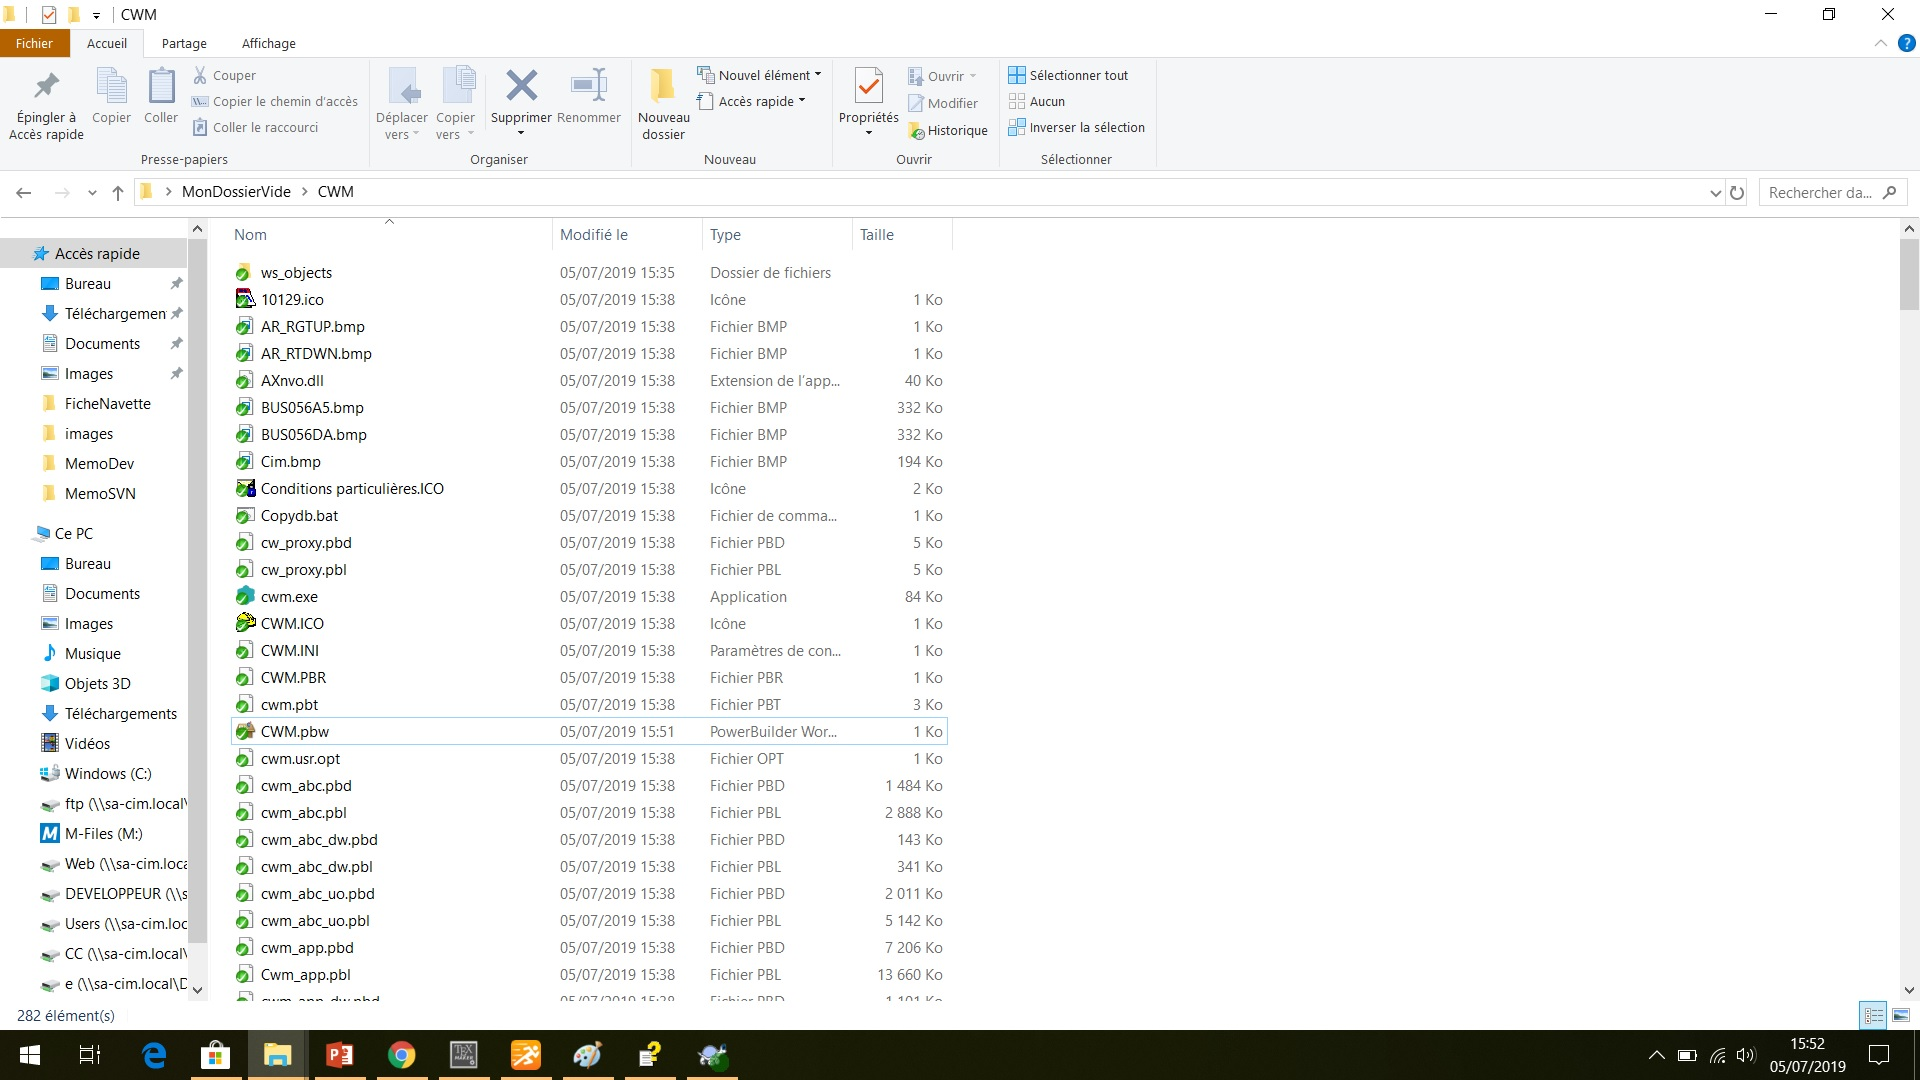
\includegraphics[scale=0.25]{../images/checkout4.jpg}
\end{frame}
\begin{frame}
\frametitle{Utilisation de TortoiseSVN}
\begin{block}{Commiter les modifications}
Pour commiter ses modifications sur le server SVN( le dépôt SVN), il faut
\begin{itemize}
\item Cliquer droit sur le projet
\item Choisir l'option \alert{\textit{SVN commit}}
\item Écrire un commentaire et appuyer sur ok.
\end{itemize}
\end{block}
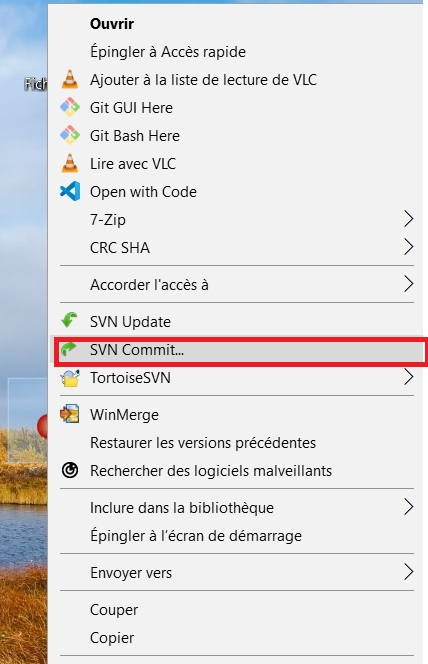
\includegraphics[scale=.3]{../images/commit5.jpg}
\end{frame}

\begin{frame}
\frametitle{Utilisation de TortoiseSVN}
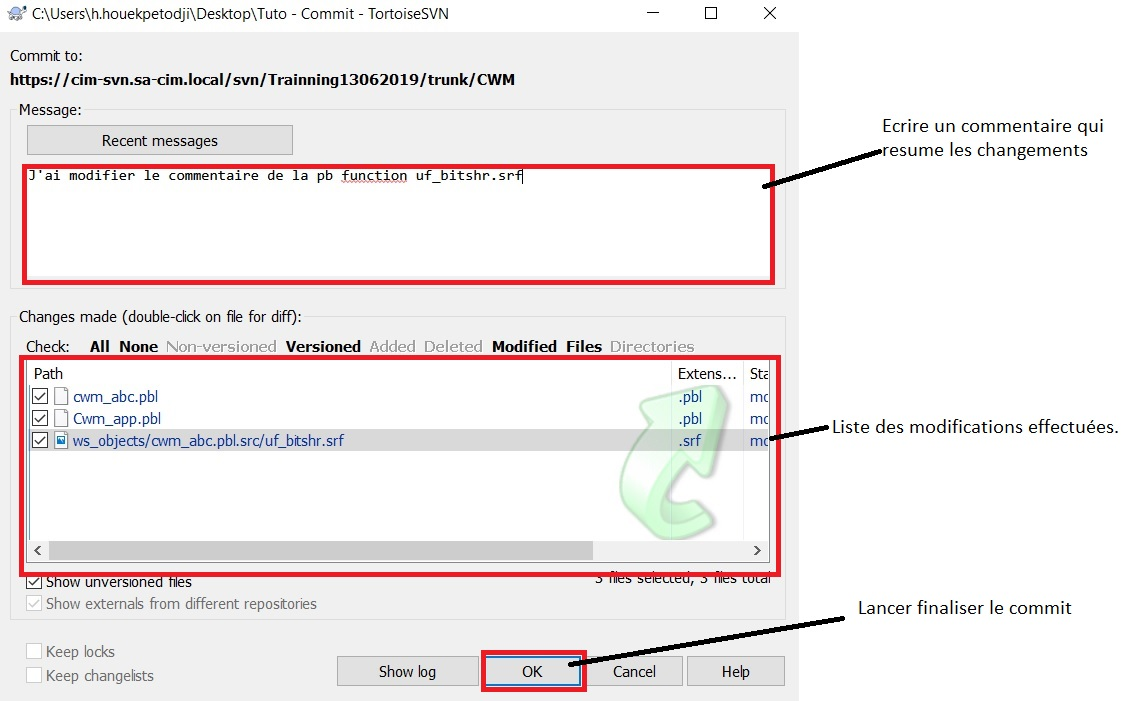
\includegraphics[scale=.4]{../images/commentaire.jpg}
\end{frame}

\begin{frame}
\begin{center}
\huge{Récupération des mises à jours du dépôt SVN}
\end{center}
\end{frame}

\begin{frame}
\frametitle{Utilisation de TortoiseSVN}
\begin{block}{Récupération des mises à jours du dépôt SVN }
Pour récupérer les mises à jours depuis le dépôt SVN, il faut avoir préalablement récupérer le projet sur sa machine via \alert{\textit{SVN checkout}} . Ensuite,
\begin{itemize}
\item Cliquer droit sur le projet,
\item Choisir l'option SVN update dans le menu.
\end{itemize} 
\end{block}
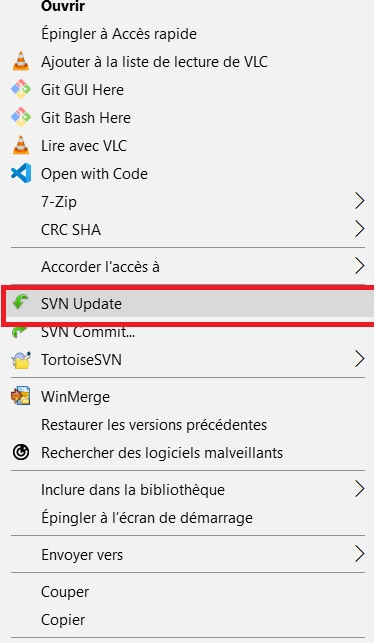
\includegraphics[scale=0.3]{../images/update1.jpg}
\end{frame}


\begin{frame}
\begin{center}
\huge{Résolution de Conflit}
\end{center}
\end{frame}

\begin{frame}
\frametitle{Utilisation de TortoiseSVN}
\begin{block}{Résolution de Conflit}
En cas de conflit, TortoiseSVN donne la main au développeur pour résoudre le conflit. La résolution du conflit suit les étapes suivantes :
\begin{itemize}
\item Cliquer droit sur le projet
\item Suivre l'option TortoiseSVN et choisir \alert{Resolve}
\end{itemize}
\end{block}
\end{frame}
\begin{frame}
\frametitle{Utilisation de TortoiseSVN}
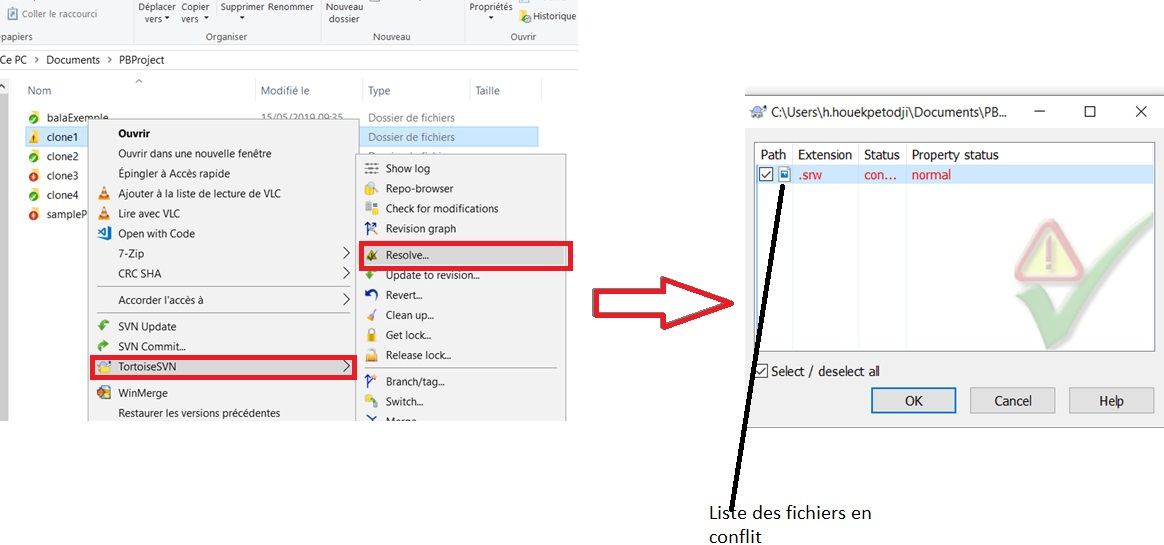
\includegraphics[scale=0.5]{../images/conflit3.jpg}
\end{frame}
\begin{frame}
\frametitle{Utilisation de TortoiseSVN}
\begin{block}{Résolution de Conflit}
\begin{itemize}
\item Cliquer droit sur les fichiers en conflit
\item Choisir l'option \alert{\textit{Edit conflit}}
\end{itemize}
\end{block}
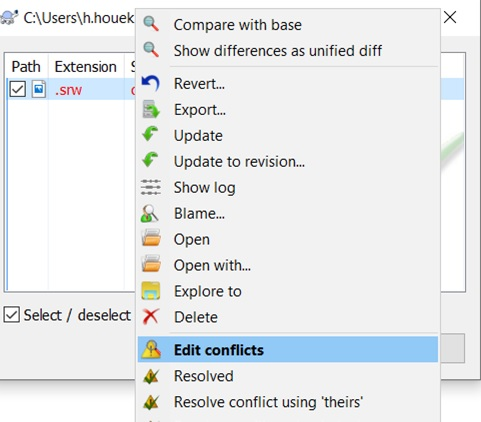
\includegraphics[scale=0.5]{../images/conflit4.jpg}
\end{frame}

\begin{frame}
\frametitle{Utilisation de TortoiseSVN}
\begin{block}{Résolution de Conflit}
La fenêtre qui se présente vous permet de résoudre le conflit manuellement. A gauche de la fenêtre, il y a la version du fichier sur le serveur SVN.  A droite, il y a la version du fichier sur votre machine. Les lignes en couleurs, indiquent les zones de conflit entre les deux versions. Dans la sous-fenêtre du bas, il y a la version finale, résultant de la résolution du conflit.  Pour résoudre le(s) conflit(s), il suffit de :
\begin{itemize}
\item Parcourir les zones de conflits avec les boutons \alert{\textit{Previous conflict}} et \alert{\textit{Next conflict}} en tête de la fenêtre.
\item Cliquer droit sur les zones de conflit. Choisir de garder ou de rejeter le contenu.
\item Cliquer sur le bouton \alert{\textit{Mark as Resolve}} et fermer la fenêtre
\item Commiter les changement sur le serveur SVN
\end{itemize}

\end{block}
\end{frame}
\begin{frame}
\frametitle{Utilisation de TortoiseSVN}
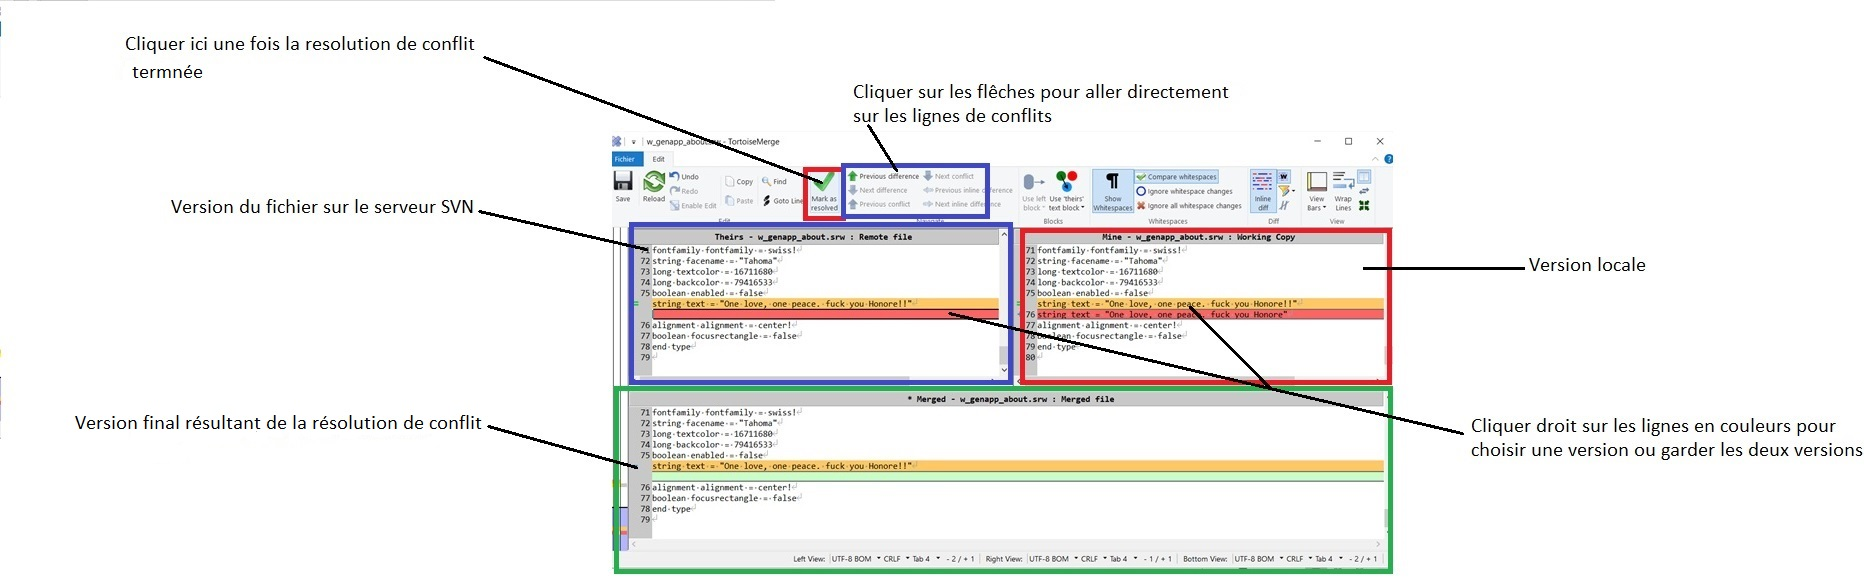
\includegraphics[scale=0.3]{../images/conflit5.jpg}
\end{frame}


\begin{frame}
\begin{center}
\huge{Modification d'une Version étiquetée}
\end{center}
\end{frame}

\begin{frame}
\frametitle{Utilisation de TortoiseSVN}

\begin{block}{Modification d'une Version étiquetée}
Souvent, après avoir arrêter (étiqueter) une version, il arrive qu'on a  besoin de faire un patch pour fixer un bug ou faire une modification particulière sur la version arrêter.  Il faut suivre les étapes suivantes pour modifier une version arrêtée:
\begin{itemize}
\item Recupérer la version étiquetée sur votre machine via l'opération \alert{\textit{SVN Checkout}} (voir slide \ref{svnCheckout} )
\item Copier la version récupérer vers \alert{\textit{branch}}:
\begin{itemize}
\item Cliquer droit sur le projet
\item Suivre l'option \alert{\textit{TortoiseSVN}} et choisir l'option \alert{\textit{Branch/tag..}}
\end{itemize}
\end{itemize}
\end{block}
\end{frame}

\begin{frame}
\frametitle{Utilisation de TortoiseSVN}
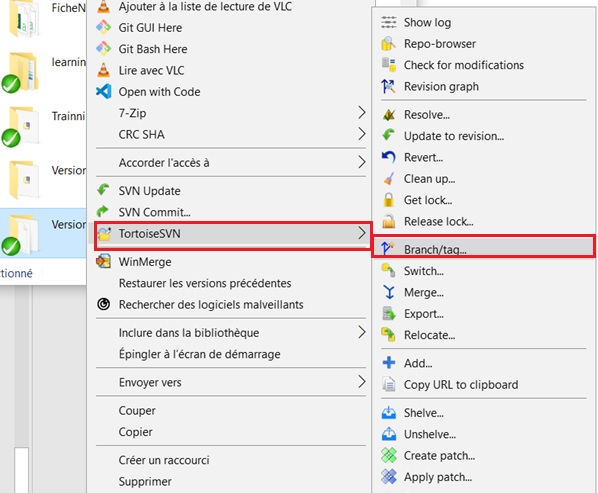
\includegraphics[scale=.7]{../images/etiquetage1.jpg}
\end{frame}

\begin{frame}
\frametitle{Utilisation de TortoiseSVN}
\begin{block}{Modification d'une Version étiquetée}
\begin{itemize}
\item Dans le champs de text correspondant à \alert{\textit{To path:}}, saisir \alert{\textit{/branches/}} suivi du nom de la version arrêtée.
\item Saisir un commentaire
\item Cliquer sur \alert{\textit{Ok}}
\end{itemize}
\end{block}
\end{frame}

\begin{frame}
\frametitle{Utilisation de TortoiseSVN}
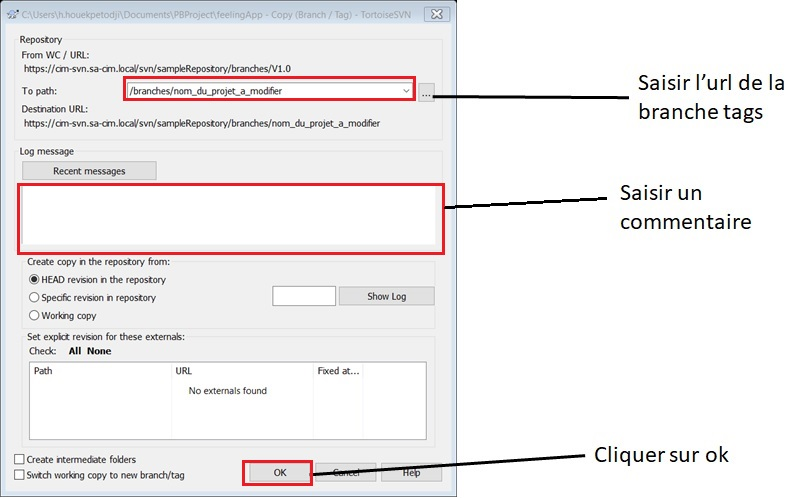
\includegraphics[scale=.7]{../images/etiquetage3.jpg}
\end{frame}

\begin{frame}
\frametitle{Utilisation de TortoiseSVN}
\begin{block}{Modification d'une Version étiquetée}
\begin{itemize}
\item Ouvrer le projet dans PowerBuilder. Faite vos modifications
\item Commiter vos modifications sur l'URL de \alert{\textit{Branches}}
\end{itemize}
\end{block}
\end{frame}

\begin{frame}
\frametitle{Résumé}
\begin{block}{Commandes résumé}
En somme  les commandes les plus courants de SVN que vous  utiliserez sont:
\begin{itemize}
\item  SVN checkout : Récupérer un projet du serveur SVN
\item SVN update : Récupérer les modifications avant de commencer à travail et pendant le travail. 
\item SVN commit : Mettre à jour le projet sur le serveur SVN avec ces modifications.
\end{itemize}
\end{block}

\end{frame}
\end{document}